\documentclass[11pt,fleqn, openany]{book} % Default font size and left-justified equations

%%%%%%%%%%%%%%%%%%%%%%%%%%%%%%%%%%%%%%%%%
% The Legrand Orange Book
% Structural Definitions File
% Version 2.1 (26/09/2018)
%
% Original author:
% Mathias Legrand (legrand.mathias@gmail.com) with modifications by:
% Vel (vel@latextemplates.com)
% 
% This file was downloaded from:
% http://www.LaTeXTemplates.com
%
% License:
% CC BY-NC-SA 3.0 (http://creativecommons.org/licenses/by-nc-sa/3.0/)
%
%%%%%%%%%%%%%%%%%%%%%%%%%%%%%%%%%%%%%%%%%

%----------------------------------------------------------------------------------------
%	VARIOUS REQUIRED PACKAGES AND CONFIGURATIONS
%----------------------------------------------------------------------------------------

\usepackage[table]{xcolor}

\usepackage{graphicx}
\usepackage{tabularx} % Required for including pictures
\usepackage{pgf,tikz,tkz-tab,eurosym,yhmath, stmaryrd}
\usepackage{pgfplots}
\usepackage{mathrsfs}
\usetikzlibrary{patterns}
\usetikzlibrary{trees}
\graphicspath{{../../Pictures/}}
\usepackage{multicol} 


\usepackage[english]{babel} % English language/hyphenation
\usepackage{icomma}
\usepackage{enumitem} % Customize lists
\setlist{nolistsep, nosep, nolistsep} % Reduce spacing between bullet points and numbered lists

\usepackage{booktabs} % Required for nicer horizontal rules in tables

 % Required for specifying colors by name


\definecolor{ocre}{RGB}{243,102,25} % Define the orange color used for highlighting throughout the book

\usepackage{listings}

\definecolor{codegreen}{rgb}{0,0.6,0}
\definecolor{codegray}{rgb}{0.5,0.5,0.5}
\definecolor{codepurple}{rgb}{0.58,0,0.82}
\definecolor{backcolour}{rgb}{0.95,0.95,0.92}

\lstdefinestyle{mystyle}{
    backgroundcolor=\color{backcolour},   
    commentstyle=\color{codegreen},
    keywordstyle=\color{magenta},
    numberstyle=\tiny\color{codegray},
    stringstyle=\color{codepurple},
    basicstyle=\ttfamily\footnotesize,
    breakatwhitespace=false,         
    breaklines=true,                 
    captionpos=b,                    
    keepspaces=true,                 
    numbers=left,                    
    numbersep=5pt,                  
    showspaces=false,                
    showstringspaces=false,
    showtabs=false,                  
    tabsize=2
}

\lstset{style=mystyle}

%----------------------------------------------------------------------------------------
% Paramétrage XSIM
%----------------------------------------------------------------------------------------

\usepackage[no-files]{xsim}


\DeclareExerciseEnvironmentTemplate{myex}{%
    \textbf{%
      \hypertarget{ex:\ExerciseID}{\sffamily{\ensuremath{\blacktriangleright}} Exercice \GetExerciseProperty{counter} \GetExerciseProperty{subtitle} --}
      \hyperlink{sol:\ExerciseID}{Voir le corrigé}%
    }\par
}{\par\smallskip}

\DeclareExerciseEnvironmentTemplate{mysol}{%
    \textbf{%
      \hypertarget{sol:\ExerciseID}{\sffamily{\ensuremath{\blacktriangleright}} Correction \GetExerciseProperty{counter} --}
      \hyperlink{ex:\ExerciseID}{Voir l'énoncé}%
    }\par
}{\par\medskip}

\xsimsetup{
  exercise/template = myex ,
  solution/template = mysol 
}

%Collection exercices

\DeclareExerciseTagging{topic}

\xsimsetup{collect}

%----------------------------------------------------------------------------------------
% SYMBOLES
%----------------------------------------------------------------------------------------

\newcommand\imCMsym[4][\mathord]{%
  \DeclareFontFamily{U} {#2}{}
  \DeclareFontShape{U}{#2}{m}{n}{
    <-6> #25
    <6-7> #26
    <7-8> #27
    <8-9> #28
    <9-10> #29
    <10-12> #210
    <12-> #212}{}
  \DeclareSymbolFont{CM#2} {U} {#2}{m}{n}
  \DeclareMathSymbol{#4}{#1}{CM#2}{#3}
}
\newcommand\alsoimCMsym[4][\mathord]{\DeclareMathSymbol{#4}{#1}{CM#2}{#3}}

\imCMsym{cmmi}{124}{\CMjmath}

\newcommand{\Oij}{(O\,;\,\vec{\imath}\,,\, \vec{\CMjmath} )}
\newcommand{\Oijk}{(O\,;\,\vec{\imath}\,,\, \vec{\CMjmath}\,,\,\vec{k})}

\newcommand\e{\mathrm{e}}
\newcommand\R{\mathbb{R}}
\newcommand\N{\mathbb{N}}


%----------------------------------------------------------------------------------------
%	MARGINS
%----------------------------------------------------------------------------------------

\usepackage{geometry} % Required for adjusting page dimensions and margins

\geometry{
	paper=a4paper, % Paper size, change to letterpaper for US letter size
	top=3cm, % Top margin
	bottom=3cm, % Bottom margin
	left=2cm, % Left margin
	right=2cm, % Right margin
	headheight=14pt, % Header height
	footskip=1.4cm, % Space from the bottom margin to the baseline of the footer
	headsep=10pt, % Space from the top margin to the baseline of the header
	%showframe, % Uncomment to show how the type block is set on the page
}

\setlength{\parindent}{0pt}
\parskip=5pt



%----------------------------------------------------------------------------------------
%	FONTS
%----------------------------------------------------------------------------------------

\usepackage{avant} % Use the Avantgarde font for headings
\usepackage{times} % Use the Times font for headings
\usepackage{mathptmx} % Use the Adobe Times Roman as the default text font together with math symbols from the Sym­bol, Chancery and Com­puter Modern fonts

%\usepackage{microtype} % Slightly tweak font spacing for aesthetics
%\usepackage[utf8]{inputenc} % Required for including letters with accents
\usepackage[T1]{fontenc} % Use 8-bit encoding that has 256 glyphs

%----------------------------------------------------------------------------------------
%	BIBLIOGRAPHY AND INDEX
%----------------------------------------------------------------------------------------

\usepackage[style=numeric,citestyle=numeric,sorting=nyt,sortcites=true,autopunct=true,babel=hyphen,hyperref=true,abbreviate=false,backref=true,backend=biber]{biblatex}
\addbibresource{bibliography.bib} % BibTeX bibliography file
\defbibheading{bibempty}{}

\usepackage{calc} % For simpler calculation - used for spacing the index letter headings correctly
\usepackage{makeidx} % Required to make an index
\makeindex % Tells LaTeX to create the files required for indexing

%----------------------------------------------------------------------------------------
%	MAIN TABLE OF CONTENTS
%----------------------------------------------------------------------------------------

\usepackage{titletoc} % Required for manipulating the table of contents

\contentsmargin{0cm} % Removes the default margin

% Part text styling (this is mostly taken care of in the PART HEADINGS section of this file)
\titlecontents{part}
	[0cm] % Left indentation
	{\addvspace{20pt}\bfseries} % Spacing and font options for parts
	{}
	{}
	{}

% Chapter text styling
\titlecontents{chapter}
	[1.25cm] % Left indentation
	{\addvspace{12pt}\large\sffamily\bfseries} % Spacing and font options for chapters
	{\color{ocre!60}\contentslabel[\Large\thecontentslabel]{1.25cm}\color{ocre}} % Formatting of numbered sections of this type
	{\color{ocre}} % Formatting of numberless sections of this type
	{\color{ocre!60}\normalsize\;\titlerule*[.5pc]{.}\;\thecontentspage} % Formatting of the filler to the right of the heading and the page number

% Section text styling
\titlecontents{section}
	[1.25cm] % Left indentation
	{\addvspace{3pt}\sffamily\bfseries} % Spacing and font options for sections
	{\contentslabel[\thecontentslabel]{1.25cm}} % Formatting of numbered sections of this type
	{} % Formatting of numberless sections of this type
	{\hfill\color{black}\thecontentspage} % Formatting of the filler to the right of the heading and the page number

% Subsection text styling
\titlecontents{subsection}
	[1.25cm] % Left indentation
	{\addvspace{1pt}\sffamily\small} % Spacing and font options for subsections
	{\contentslabel[\thecontentslabel]{1.25cm}} % Formatting of numbered sections of this type
	{} % Formatting of numberless sections of this type
	{\ \titlerule*[.5pc]{.}\;\thecontentspage} % Formatting of the filler to the right of the heading and the page number

% Figure text styling
\titlecontents{figure}
	[1.25cm] % Left indentation
	{\addvspace{1pt}\sffamily\small} % Spacing and font options for figures
	{\thecontentslabel\hspace*{1em}} % Formatting of numbered sections of this type
	{} % Formatting of numberless sections of this type
	{\ \titlerule*[.5pc]{.}\;\thecontentspage} % Formatting of the filler to the right of the heading and the page number

% Table text styling
\titlecontents{table}
	[1.25cm] % Left indentation
	{\addvspace{1pt}\sffamily\small} % Spacing and font options for tables
	{\thecontentslabel\hspace*{1em}} % Formatting of numbered sections of this type
	{} % Formatting of numberless sections of this type
	{\ \titlerule*[.5pc]{.}\;\thecontentspage} % Formatting of the filler to the right of the heading and the page number

%----------------------------------------------------------------------------------------
%	MINI TABLE OF CONTENTS IN PART HEADS
%----------------------------------------------------------------------------------------

% Chapter text styling
\titlecontents{lchapter}
	[0em] % Left indentation
	{\addvspace{15pt}\large\sffamily\bfseries} % Spacing and font options for chapters
	{\color{ocre}\contentslabel[\Large\thecontentslabel]{1.25cm}\color{ocre}} % Chapter number
	{}  
	{\color{ocre}\normalsize\sffamily\bfseries\;\titlerule*[.5pc]{.}\;\thecontentspage} % Page number

% Section text styling
\titlecontents{lsection}
	[0em] % Left indentation
	{\sffamily\small} % Spacing and font options for sections
	{\contentslabel[\thecontentslabel]{1.25cm}} % Section number
	{}
	{}

% Subsection text styling (note these aren't shown by default, display them by searchings this file for tocdepth and reading the commented text)
\titlecontents{lsubsection}
	[.5em] % Left indentation
	{\sffamily\footnotesize} % Spacing and font options for subsections
	{\contentslabel[\thecontentslabel]{1.25cm}}
	{}
	{}

%----------------------------------------------------------------------------------------
%	HEADERS AND FOOTERS
%----------------------------------------------------------------------------------------


\usepackage{fancyhdr} % Required for header and footer configuration

\pagestyle{fancy}
\renewcommand{\chaptermark}[1]{\markboth{\sffamily\normalsize\bfseries\ \thechapter.\ #1}{}} % Chapter text font settings
\renewcommand{\sectionmark}[1]{\markright{\sffamily\normalsize\thesection\hspace{5pt}#1}{}} % Section text font settings
\fancyhf{} \fancyhead[LE,RO]{\sffamily\normalsize\thepage} % Font setting for the page number in the header
\fancyhead[LO]{\rightmark} % Print the nearest section name on the left side of odd pages
\fancyhead[RE]{\leftmark} % Print the current chapter name on the right side of even pages

\fancyfoot[L]{Jason LAPEYRONNIE}
\fancyfoot[R]{\href{http://mathoutils.fr}{http://mathoutils.fr}} % Uncomment to include a footer

\renewcommand{\headrulewidth}{0.5pt} % Thickness of the rule under the header
\renewcommand{\footrulewidth}{0.5pt} % Thickness of the rule under the header

\fancypagestyle{plain}{% Style for when a plain pagestyle is specified
	\fancyhead{}\renewcommand{\headrulewidth}{0pt}%
}

% Removes the header from odd empty pages at the end of chapters
\makeatletter
\renewcommand{\cleardoublepage}{
\clearpage\ifodd\c@page\else
\hbox{}
\vspace*{\fill}
\thispagestyle{empty}
\newpage
\fi}

%----------------------------------------------------------------------------------------
%	THEOREM STYLES
%----------------------------------------------------------------------------------------

\usepackage{amsmath,amsfonts,amssymb,amsthm} % For math equations, theorems, symbols, etc

\newcommand{\intoo}[2]{\mathopen{]}#1\,;#2\mathclose{[}}
\newcommand{\ud}{\mathop{\mathrm{{}d}}\mathopen{}}
\newcommand{\intff}[2]{\mathopen{[}#1\,;#2\mathclose{]}}
\renewcommand{\qedsymbol}{$\blacksquare$}
\newtheorem{notation}{Notation}[section]

% Boxed/framed environments
\newtheoremstyle{ocrenumbox}% Theorem style name
{0pt}% Space above
{0pt}% Space below
{\normalfont}% Body font
{}% Indent amount
{\small\bf\sffamily\color{ocre}}% Theorem head font
{\;:\;}% Punctuation after theorem head
{0.25em}% Space after theorem head
{\small\sffamily\color{ocre}\thmname{#1}\nobreakspace\thmnumber{\@ifnotempty{#1}{}\@upn{#2}}% Theorem text (e.g. Theorem 2.1)
\thmnote{\nobreakspace\the\thm@notefont\sffamily\bfseries\color{black}---\nobreakspace#3}} % Optional theorem note

\newtheoremstyle{blacknumex}% Theorem style name
{5pt}% Space above
{10pt}% Space below
{\normalfont}% Body font
{} % Indent amount
{\small\bf\sffamily}% Theorem head font
{\;:\;}% Punctuation after theorem head
{0.25em}% Space after theorem head
{\small\sffamily{\tiny\ensuremath{\blacksquare}}\nobreakspace\thmname{#1}\nobreakspace\thmnumber{\@ifnotempty{#1}{}\@upn{#2}}% Theorem text (e.g. Theorem 2.1)
\thmnote{\nobreakspace\the\thm@notefont\sffamily\bfseries---\nobreakspace#3}}% Optional theorem note

\newtheoremstyle{blacknumexo}% Theorem style name
{15pt}% Space above
{10pt}% Space below
{\normalfont}% Body font
{} % Indent amount
{\small\bf\sffamily}% Theorem head font
{}% Punctuation after theorem head
{0.5em}% Space after theorem head
{\small\sffamily{\ensuremath{\blacktriangleright}}\nobreakspace\thmname{#1}\nobreakspace\thmnumber{\@ifnotempty{#1}{}\@upn{#2}}% Theorem text (e.g. Theorem 2.1)
\thmnote{\nobreakspace\the\thm@notefont\sffamily\bfseries---\nobreakspace#3} \\}% Optional theorem note



\newtheoremstyle{blacknumbox} % Theorem style name
{0pt}% Space above
{5pt}% Space below
{}% Body font
{}% Indent amount
{\large\bf\sffamily}% Theorem head font
{\;:\;}% Punctuation after theorem head
{0.25em}% Space after theorem head
{\small\sffamily\thmname{#1}\nobreakspace\thmnumber{\@ifnotempty{#1}{}\@upn{#2}}% Theorem text (e.g. Theorem 2.1)
\thmnote{\nobreakspace\the\thm@notefont\sffamily\bfseries---\nobreakspace#3}}% Optional theorem note

% Non-boxed/non-framed environments
\newtheoremstyle{ocrenum}% Theorem style name
{5pt}% Space above
{5pt}% Space below
{\normalfont}% Body font
{}% Indent amount
{\small\bf\sffamily\color{ocre}}% Theorem head font
{\;:\;}% Punctuation after theorem head
{0.25em}% Space after theorem head
{\small\sffamily\color{ocre}\thmname{#1}\nobreakspace\thmnumber{\@ifnotempty{#1}{}\@upn{#2}}% Theorem text (e.g. Theorem 2.1)
\thmnote{\nobreakspace\the\thm@notefont\sffamily\bfseries\color{black}---\nobreakspace#3}} % Optional theorem note
\makeatother

% Defines the theorem text style for each type of theorem to one of the three styles above
\newcounter{dummy} 
\newcounter{thm}
\newcounter{correction}
\newcounter{qst}
\theoremstyle{ocrenumbox}
\newtheorem{theoremeT}[dummy]{Théorème}
\newtheorem{exerciseT}{Propriété}
\newtheorem{principeT}{Principe}
\theoremstyle{blacknumex}
\newtheorem{exampleT}{Exemple}
\theoremstyle{blacknumexo}
\newtheorem{exo}[thm]{Exercice}
\newtheorem{corr}[correction]{Correction}
\newtheorem{quest}[qst]{Question}
\theoremstyle{blacknumbox}
\newtheorem{vocabulary}{Vocabulary}[section]
\newtheorem{definitionT}{Définition}
\newtheorem{corollaryT}[dummy]{Corollary}
\theoremstyle{ocrenum}
\newtheorem{proofT}[dummy]{Démonstration}


%----------------------------------------------------------------------------------------
%	DEFINITION OF COLORED BOXES
%----------------------------------------------------------------------------------------

\RequirePackage[framemethod=default]{mdframed} % Required for creating the theorem, definition, exercise and corollary boxes

% Theorem box
\newmdenv[skipabove=7pt,
skipbelow=7pt,
backgroundcolor=black!5,
linecolor=ocre,
innerleftmargin=5pt,
innerrightmargin=5pt,
innertopmargin=10pt,
leftmargin=0cm,
rightmargin=0cm,
innerbottommargin=5pt]{tBox}

%Proposition box	  
\newmdenv[skipabove=7pt,
skipbelow=7pt,
rightline=false,
leftline=true,
topline=false,
bottomline=false,
backgroundcolor=ocre!10,
linecolor=ocre,
innerleftmargin=5pt,
innerrightmargin=5pt,
innertopmargin=10pt,
innerbottommargin=3pt,
leftmargin=0cm,
rightmargin=0cm,
linewidth=4pt]{eBox}	

% Definition box
\newmdenv[skipabove=7pt,
backgroundcolor=ocre!4,
skipbelow=7pt,
rightline=false,
leftline=true,
topline=false,
bottomline=false,
linecolor=ocre,
innerleftmargin=5pt,
innerrightmargin=5pt,
innertopmargin=10pt,
leftmargin=0cm,
rightmargin=0cm,
linewidth=4pt,
innerbottommargin=5pt]{dBox}	

% Corollary box
\newmdenv[skipabove=7pt,
skipbelow=7pt,
rightline=false,
leftline=true,
topline=false,
bottomline=false,
linecolor=gray,
backgroundcolor=black!5,
innerleftmargin=5pt,
innerrightmargin=5pt,
innertopmargin=5pt,
leftmargin=0cm,
rightmargin=0cm,
linewidth=4pt,
innerbottommargin=5pt]{cBox}

\newmdenv[skipabove=7pt,
skipbelow=7pt,
backgroundcolor=black!5,
innerleftmargin=5pt,
topline=false,
bottomline=false,
rightline=false,
leftline=false,
innerrightmargin=5pt,
innertopmargin=5pt,
leftmargin=0cm,
rightmargin=0cm,
innerbottommargin=5pt]{xBox}

% Creates an environment for each type of theorem and assigns it a theorem text style from the "Theorem Styles" section above and a colored box from above
\newenvironment{theorem}{\begin{tBox}\begin{theoremeT}}{\end{theoremeT}\end{tBox}}

\newenvironment{exo2}{\noindent \begin{exo}\item\relax \noindent \begin{eBox}\item\relax}{\end{eBox}\end{exo}}


\newenvironment{proposition}{\begin{eBox}\begin{exerciseT}}{\hfill{\color{ocre}}\end{exerciseT}\end{eBox}}		

\newenvironment{principe}{\begin{eBox}\begin{principeT}}{\hfill{\color{ocre}}\end{principeT}\end{eBox}}	
		  
\newenvironment{definition}{\begin{dBox}\begin{definitionT}}{\end{definitionT}\end{dBox}}	

\newenvironment{example}{\begin{xBox}\begin{exampleT}}{\hfill{\tiny\ensuremath{\blacksquare}}\end{exampleT}\end{xBox}}

\newenvironment{demonstration}{\begin{proofT}}{\hfill{\tiny\ensuremath{\square}}\end{proofT}}		
\newenvironment{corollary}{\begin{cBox}\begin{corollaryT}}{\end{corollaryT}\end{cBox}}	

%----------------------------------------------------------------------------------------
%	REMARK ENVIRONMENT
%----------------------------------------------------------------------------------------

\newenvironment{remark}{\par\vspace{5pt}\small % Vertical white space above the remark and smaller font size
\begin{list}{}{
\leftmargin=25pt % Indentation on the left
\rightmargin=15pt}\item\ignorespaces % Indentation on the right
\makebox[-2.5pt]{
\begin{tikzpicture}[overlay]
\node[draw=ocre!60,line width=1pt,circle,fill=ocre!25,font=\sffamily\bfseries,inner sep=2pt,outer sep=0pt] at (-15pt,0pt){\textcolor{ocre}{R}};\end{tikzpicture}} % Orange R in a circle
\advance\baselineskip -1pt}{\end{list}\vskip5pt} % Tighter line spacing and white space after remark

%----------------------------------------------------------------------------------------
%	SECTION NUMBERING IN THE MARGIN
%----------------------------------------------------------------------------------------

\makeatletter
\renewcommand{\@seccntformat}[1]{\llap{\textcolor{ocre}{\csname the#1\endcsname}\hspace{1em}}}                    
\renewcommand{\section}{\@startsection{section}{1}{\z@}
{-4ex \@plus -1ex \@minus -.4ex}
{1ex \@plus.2ex }
{\normalfont\LARGE\sffamily\bfseries}}
\renewcommand{\subsection}{\@startsection {subsection}{2}{\z@}
{-3ex \@plus -0.1ex \@minus -.4ex}
{0.5ex \@plus.2ex }
{\normalfont\sffamily\bfseries}}
\renewcommand{\subsubsection}{\@startsection {subsubsection}{3}{\z@}
{-2ex \@plus -0.1ex \@minus -.2ex}
{.2ex \@plus.2ex }
{\normalfont\small\sffamily\bfseries}}                        
\renewcommand\paragraph{\@startsection{paragraph}{4}{\z@}
{-2ex \@plus-.2ex \@minus .2ex}
{.1ex}
{\normalfont\small\sffamily\bfseries}}

%----------------------------------------------------------------------------------------
%	PART HEADINGS
%----------------------------------------------------------------------------------------

% Numbered part in the table of contents
\newcommand{\@mypartnumtocformat}[2]{%
	\setlength\fboxsep{0pt}%
	\noindent\colorbox{ocre!20}{\strut\parbox[c][.7cm]{\ecart}{\color{ocre!70}\Large\sffamily\bfseries\centering#1}}\hskip\esp\colorbox{ocre!40}{\strut\parbox[c][.7cm]{\linewidth-\ecart-\esp}{\Large\sffamily\centering#2}}%
}

% Unnumbered part in the table of contents
\newcommand{\@myparttocformat}[1]{%
	\setlength\fboxsep{0pt}%
	\noindent\colorbox{ocre!40}{\strut\parbox[c][.7cm]{\linewidth}{\Large\sffamily\centering#1}}%
}

\newlength\esp
\setlength\esp{4pt}
\newlength\ecart
\setlength\ecart{1.2cm-\esp}
\newcommand{\thepartimage}{}%
\newcommand{\partimage}[1]{\renewcommand{\thepartimage}{#1}}%
\def\@part[#1]#2{%
\ifnum \c@secnumdepth >-2\relax%
\refstepcounter{part}%
\addcontentsline{toc}{part}{\texorpdfstring{\protect\@mypartnumtocformat{\thepart}{#1}}{\partname~\thepart\ ---\ #1}}
\else%
\addcontentsline{toc}{part}{\texorpdfstring{\protect\@myparttocformat{#1}}{#1}}%
\fi%
\startcontents%
\markboth{}{}%
{\thispagestyle{empty}%
\begin{tikzpicture}[remember picture,overlay]%
\node at (current page.north west){\begin{tikzpicture}[remember picture,overlay]%	
\fill[ocre!20](0cm,0cm) rectangle (\paperwidth,-\paperheight);
\node[anchor=north] at (4cm,-3.25cm){\color{ocre!40}\fontsize{220}{100}\sffamily\bfseries\thepart}; 
\node[anchor=south east] at (\paperwidth-1cm,-\paperheight+1cm){\parbox[t][][t]{8.5cm}{
\printcontents{l}{0}{\setcounter{tocdepth}{1}}% The depth to which the Part mini table of contents displays headings; 0 for chapters only, 1 for chapters and sections and 2 for chapters, sections and subsections
}};
\node[anchor=north east] at (\paperwidth-1.5cm,-3.25cm){\parbox[t][][t]{15cm}{\strut\raggedleft\color{white}\fontsize{30}{30}\sffamily\bfseries#2}};
\end{tikzpicture}};
\end{tikzpicture}}%
\@endpart}
\def\@spart#1{%
\startcontents%
\phantomsection
{\thispagestyle{empty}%
\begin{tikzpicture}[remember picture,overlay]%
\node at (current page.north west){\begin{tikzpicture}[remember picture,overlay]%	
\fill[ocre!20](0cm,0cm) rectangle (\paperwidth,-\paperheight);
\node[anchor=north east] at (\paperwidth-1.5cm,-3.25cm){\parbox[t][][t]{15cm}{\strut\raggedleft\color{white}\fontsize{30}{30}\sffamily\bfseries#1}};
\end{tikzpicture}};
\end{tikzpicture}}
\addcontentsline{toc}{part}{\texorpdfstring{%
\setlength\fboxsep{0pt}%
\noindent\protect\colorbox{ocre!40}{\strut\protect\parbox[c][.7cm]{\linewidth}{\Large\sffamily\protect\centering #1\quad\mbox{}}}}{#1}}%
\@endpart}
\def\@endpart{\vfil\newpage
\if@twoside
\if@openright
\null
\thispagestyle{empty}%
\newpage
\fi
\fi
\if@tempswa
\twocolumn
\fi}

%----------------------------------------------------------------------------------------
%	CHAPTER HEADINGS
%----------------------------------------------------------------------------------------

% A switch to conditionally include a picture, implemented by Christian Hupfer
\newif\ifusechapterimage
\usechapterimagetrue
\newcommand{\thechapterimage}{}%
\newcommand{\chapterimage}[1]{\ifusechapterimage\renewcommand{\thechapterimage}{#1}\fi}%
\newcommand{\autodot}{.}
\def\@makechapterhead#1{%
{\parindent \z@ \raggedright \normalfont
\ifnum \c@secnumdepth >\m@ne
\if@mainmatter
\begin{tikzpicture}[remember picture,overlay]
\node at (current page.north west)
{\begin{tikzpicture}[remember picture,overlay]
\node[anchor=north west,inner sep=0pt] at (0,0) {\ifusechapterimage\includegraphics[width=\paperwidth]{\thechapterimage}\fi};
\draw[anchor=west] (\Gm@lmargin,-3cm) node [line width=2pt,rounded corners=15pt,draw=ocre,fill=white,fill opacity=0.5,inner sep=15pt]{\strut\makebox[22cm]{}};
\draw[anchor=west] (\Gm@lmargin+.3cm,-3cm) node {\huge\sffamily\bfseries\color{black}\thechapter\autodot~#1\strut};
\end{tikzpicture}};
\end{tikzpicture}
\else
\begin{tikzpicture}[remember picture,overlay]
\node at (current page.north west)
{\begin{tikzpicture}[remember picture,overlay]
\node[anchor=north west,inner sep=0pt] at (0,0) {\ifusechapterimage\includegraphics[width=\paperwidth]{\thechapterimage}\fi};
\draw[anchor=west] (\Gm@lmargin,-3cm) node [line width=2pt,rounded corners=15pt,draw=ocre,fill=white,fill opacity=0.5,inner sep=15pt]{\strut\makebox[22cm]{}};
\draw[anchor=west] (\Gm@lmargin+.3cm,-3cm) node {\huge\sffamily\bfseries\color{black}#1\strut};
\end{tikzpicture}};
\end{tikzpicture}
\fi\fi\par\vspace*{50\p@}}}

%-------------------------------------------

\def\@makeschapterhead#1{%
\begin{tikzpicture}[remember picture,overlay]
\node at (current page.north west)
{\begin{tikzpicture}[remember picture,overlay]
\node[anchor=north west,inner sep=0pt] at (0,0) {\ifusechapterimage\includegraphics[width=\paperwidth]{\thechapterimage}\fi};
\draw[anchor=west] (\Gm@lmargin,-3cm) node [line width=2pt,rounded corners=15pt,draw=ocre,fill=white,fill opacity=0.5,inner sep=15pt]{\strut\makebox[22cm]{}};
\draw[anchor=west] (\Gm@lmargin+.3cm,-3cm) node {\huge\sffamily\bfseries\color{black}#1\strut};
\end{tikzpicture}};
\end{tikzpicture}
\par\vspace*{50\p@}}
\makeatother

%----------------------------------------------------------------------------------------
%	LINKS
%----------------------------------------------------------------------------------------

\usepackage{hyperref}
\hypersetup{hidelinks,backref=true,pagebackref=true,hyperindex=true,colorlinks=false,breaklinks=true,urlcolor=ocre,bookmarks=true,bookmarksopen=false}

\usepackage{bookmark}
\bookmarksetup{
open,
numbered,
addtohook={%
\ifnum\bookmarkget{level}=0 % chapter
\bookmarksetup{bold}%
\fi
\ifnum\bookmarkget{level}=-1 % part
\bookmarksetup{color=ocre,bold}%
\fi
}
}

\renewcommand*\thesection{\arabic{section}}

\newcommand*{\coord}[3]{% 
  \ensuremath{\overrightarrow{#1}\, 
    \begin{pmatrix} 
      #2\\ 
      #3 
    \end{pmatrix}}}
    
  \newcommand*{\coordb}[2]{% 
  \ensuremath{ 
    \begin{pmatrix} 
      #1\\ 
      #2 
    \end{pmatrix}}}

\newcommand*{\coorde}[4]{% 
  \renewcommand{\arraystretch}{1}\ensuremath{\overrightarrow{#1}\, 
    \begin{pmatrix} 
      #2\\ 
      #3 \\
      #4
    \end{pmatrix}}}    
  \newcommand*{\coordbe}[3]{% 
 \renewcommand{\arraystretch}{1} \ensuremath{ 
    \begin{pmatrix} 
      #1\\ 
      #2 \\
      #3
    \end{pmatrix}}}  
    
\newcommand{\Card}{\mathrm{Card}}




\begin{document}

\chapterimage{../../Pictures/background}


\chapter{Cours : Loi binomiale}


\section{Succession d'épreuves indépendantes}



\begin{definition}[Succession d'épreuves]Soit $n$ un entier naturel. On considère $n$ épreuves aléatoires dont les univers sont respectivement $\Omega_1$, $\Omega_2$, ... , $\Omega_n$.

L'univers $\Omega$ de la succession de ces $n$ épreuves est le produit cartésien $\Omega_1 \times \Omega_2 \times \dots \times \Omega_n$.

Les issues de cette succession d'expériences sont les $n$-uplets $(i_1\, ;\, i_2\,;\,\dots\,;\,i_n)$ de $\Omega_1 \times \Omega_2 \times \dots \times \Omega_n$.\end{definition}

\begin{example}On lance 2 fois un dé à 6 faces, numérotées de $1$ à $6$ et on regarde le numéro obtenu. L'univers de cette expérience est $\{1;2;3;4;5;6\}^2$. L'issue $(1\,;\,3)$ signifie que l'on a obtenu 1 au premier lancer et 3 au deuxième.\end{example}

\begin{definition}[Indépendance mutuelle]Soit $n$ un entier naturel. On considère $n$ épreuves aléatoires dont les univers sont respectivement $\Omega_1$, $\Omega_2$, ... , $\Omega_n$, de lois respectives $\mathbb{P}_1$, $\mathbb{P}_2$, ... , $\mathbb{P}_n$.

Les épreuves sont dites mutuellement indépendantes (ou tout simplement indépendantes) si, pour toute issue $(i_1,i_2,...,i_n)$ de $\Omega_1 \times \Omega_2 \times \dots \times \Omega_n$, on a
\[ \mathbb{P}((i_1,i_2,...,i_n))=\mathbb{P}_1(i_1) \times \mathbb{P}_2(i_2) \times \dots \times \mathbb{P}_n(i_n).\]
Autrement dit, la probabilité d'une issue est égale au produit des probabilités de chacune des composantes $i_1$, $i_2$, ..., $i_n$.\end{definition}

\begin{example}M. Lapeyronnie a décidé de faire un petit contrôle surprise à ses élèves. Il place les noms des élèves de la classe dans une urne et une liste d'exercices dans une autre. 
\begin{itemize}
\item Il y a 29 élèves dans la classe. Parmi eux, 12 suivent l'option Maths expertes ;
\item L'urne des exercices en contient 40 : 20 sur les fonctions, 15 sur les suites et 5 sur la géométrie.
\end{itemize}
M. Lapeyronnie tire alors simultanément, de manière indépendante, un nom d'élève et un exercice.

\begin{itemize}
\item La probabilité qu'il s'agisse d'un élève suivant l'option Maths expertes est de $\dfrac{12}{29}$ ;
\vskip10pt
\item La probabilité de tirer un exercice de géométrie est de $\dfrac{5}{40}=\dfrac{1}{8}$ ;
\vskip10pt
\item La probabilité qu'un élève suivant l'option Maths Expertes soit envoyé au tableau faire un exercice de géométrie est donc de $\dfrac{12}{29} \times \dfrac{1}{8} = \dfrac{3}{58}$.
\end{itemize}
\end{example}

Si l'on essaie de représenter une succession de $n$ épreuves indépendantes sous la forme d'un arbre de probabilités, on place alors toujours le même sous-arbre à chaque noeud d'un étage fixé. De plus, cet arbre peut être construit "dans un sens comme dans l'autre".
\newpage
\begin{example}Les arbres suivants traduisent la succession des deux épreuves précédentes. 


\noindent\begin{minipage}{0.49\linewidth}
\tikzstyle{level 1}=[level distance=3.5cm, sibling distance=5cm]
\tikzstyle{level 2}=[level distance=3.5cm, sibling distance=2cm]
\tikzstyle{level 3}=[level distance=3.5cm, sibling distance=0.3cm]

% Define styles for bags and leafs
\tikzstyle{bag} = []
\tikzstyle{end} = [circle, minimum width=3pt,fill, inner sep=0pt]


\begin{center}
\begin{tikzpicture}[scale=0.8,grow=right,sloped]
\node[bag] { }
	child {
        node[bag] {Maths Exp.} 
        child {
                node[bag] {Géométrie}
                edge from parent node[below] {$1/8$}
            }
        child {
               node[bag] {Suites}
               edge from parent node[above] {$3/8$}
            }
        child {
                node[bag] {Fonctions}
                edge from parent node[above] {$1/2$}
            }
            edge from parent node[above] {$12/29$} 
    }
	child {
        node[bag] {Pas Maths Exp.} 
        child {
                node[bag] {Géométrie}
                edge from parent node[below] {$1/8$}
            }
        child {
               node[bag] {Suites}
               edge from parent node[above] {$3/8$}
            }
        child {
                node[bag] {Fonctions}
                edge from parent node[above] {$1/2$}
            }
            edge from parent node[above] {$17/29$}  
    };
\end{tikzpicture}
\end{center}
\end{minipage} \begin{minipage}{0.49\linewidth}
\tikzstyle{level 1}=[level distance=3.5cm, sibling distance=3cm]
\tikzstyle{level 2}=[level distance=5cm, sibling distance=2cm]
\tikzstyle{level 3}=[level distance=3.5cm, sibling distance=0.3cm]

% Define styles for bags and leafs
\tikzstyle{bag} = []
\tikzstyle{end} = [circle, minimum width=3pt,fill, inner sep=0pt]


\begin{center}
\begin{tikzpicture}[scale=0.8,grow=right,sloped]
\node[bag] { }
	child {
        node[bag] {Géométrie} 
        child {
                node[bag] {Maths Exp.}
                edge from parent node[below] {$12/29$}
            }
        child {
               node[bag] {Pas Maths Exp.}
               edge from parent node[above] {$17/29$}
            }
            edge from parent node[above] {$1/8$} 
    }
	child {
        node[bag] {Suites} 
        child {
                node[bag] {Maths Exp.}
                edge from parent node[below] {$12/29$}
            }
        child {
               node[bag] {Pas Maths Exp.}
               edge from parent node[above] {$17/29$}
            }
            edge from parent node[above] {$3/8$} 
    }
    child {
        node[bag] {Fonctions} 
        child {
                node[bag] {Maths Exp.}
                edge from parent node[below] {$12/29$}
            }
        child {
               node[bag] {Pas Maths Exp.}
               edge from parent node[above] {$17/29$}
            }
            edge from parent node[above] {$1/2$} 
    };
\end{tikzpicture}
\end{center}
\end{minipage}

\end{example}

\begin{example}Soit $n$ un entier naturel. On lance $n$ fois un dé équilibré à six faces, numérotées de 1 à 6.

La probabilité de ne jamais obtenir le résultat 6 sur ces $n$ lancers est alors de $\left(\dfrac{5}{6}\right)^n$. Ainsi, la probabilité d'obtenir une au moins une fois le résultat 6 sur ces $n$ lancers vaut donc $1-\left(\dfrac{5}{6}\right)^n$.

Par ailleurs, puisque $-1< \dfrac{5}{6}<1$, on a $\displaystyle\lim_{n \to +\infty}\left(\dfrac{5}{6}\right)^n=0$ et donc $\displaystyle\lim_{n \to +\infty}\left(1-\left(\dfrac{5}{6}\right)^n\right)=1$.

Si l'on lance un grand nombre de fois un dé classique à six faces, la probabilité d'obtenir au moins une fois le résultat 6 est proche de 1.

On peut alors se demander combien de lances effectuer pour que cette probabilité dépasse 0,99. On cherche alors l'entier $n$ à partir duquel $1-\left(\dfrac{5}{6}\right)^n \geqslant 0,99$.

On a alors $-\left(\dfrac{5}{6}\right)^n \geqslant -0,01$ soit $\left(\dfrac{5}{6}\right)^n \leqslant 0,01$. On applique alors la fonction logarithme népérien qui est croissante sur $]0;+\infty[$. On a donc $n\ln\left(\dfrac{5}{6}\right)\leqslant \ln(0,01)$. On divise alors par $\ln\left(\dfrac{5}{6}\right)$ qui est négatif, on aboutit à $n\geqslant \dfrac{\ln(0,01)}{\ln\left(\frac{5}{6}\right)}$. Or, $ \dfrac{\ln(0,01)}{\ln\left(\frac{5}{6}\right)}\simeq 25,3$.

 Ainsi, à partir de 26 lancers de dés à six faces, on est certains à au moins 99\% d'obtenir au moins une fois le résultat 6.
\end{example}

\newpage 
\section{Epreuve de Bernoulli}

\begin{definition}[Epreuve de Bernoulli]Une épreuve de Bernoulli est une expérience aléatoire dont l'univers ne comporte que deux issues : le succès $S$ et l'échec $\overline{S}$. On note $p$ la probabilité de succès, aussi appelé paramètre de l'épreuve de Bernoulli. La probabilité d'échec vaut donc $1-p$.

Une variable aléatoire $X$ sur cet univers suit une loi de Bernoulli de paramètre $p$ si on a $\mathbb{P}(X=1)=p$ et $\mathbb{P}(X=0)=1-p$. On écrit $X \sim \mathcal{B}(p)$.\end{definition}


\noindent\begin{minipage}{0.49\linewidth}
\begin{center}
\textbf{Epreuve de Bernoulli}
\renewcommand{\arraystretch}{1.2}
\begin{tabularx}{0.8\linewidth}{|X|X|X|}
\hline
Issue & $S$ & $\overline{S}$\\
\hline
Proba & $p$ & $1-p$\\
\hline
\end{tabularx}
\end{center}
\end{minipage}\hfill\begin{minipage}{0.49\linewidth}
\begin{center}
\textbf{Variable de Bernoulli}
\renewcommand{\arraystretch}{1.2}
\begin{tabularx}{0.8\linewidth}{|X|X|X|}
\hline
$k$ & 1 & 0\\
\hline
$\mathbb{P}(X=k)$ & $p$ & $1-p$\\
\hline
\end{tabularx}
\end{center}
\end{minipage}



\begin{example}On lance un dé équilibré à 6 faces, numérotées de 1 à 6. Si on considère le succès "Obtenir le nombre 6", cette expérience est une épreuve de Bernoulli de paramètre $p=\dfrac{1}{6}$. \end{example}

\begin{proposition}Soit $X$ une variable aléatoire suivant une loi de Bernoulli de paramètre $p$. L'espérance, la variance et l'écart-type de $X$ valent respectivement \[E[X]=p, \quad V(X)=p(1-p), \quad \sigma(X)=\sqrt{p(1-p)}\]\end{proposition}



\begin{demonstration} La variable aléatoire $X$ prend les valeurs 0 et 1. De plus $\mathbb{P}(X=0)=1-p$ et \\ $\mathbb{P}(X=1)=p$. Ainsi,
\[E[X] = 0 \times \mathbb{P}(X=0)+1 \times \mathbb{P}(X=1)=0 \times (1-p)+1 \times p = p\]
et
\[V(X)=\mathbb{P}(X=0) \times (0- E[X])^2 + \mathbb{P}(X=1) \times (1- E[X])^2\]
d'où
\[V(X)=(1-p) \times (-p)^2+p \times (1-p)^2=p(1-p)(p+1-p)=p(1-p).\]
\end{demonstration}

\begin{demonstration}[Avec la formule de Koenig-Huygens]
On sait que $V(X)=E[X^2]-(E[X])^2$.

Or, la variable aléatoire $X$ vaut soit 0, soit 1. Par ailleurs, $0^2=0$ et $1^2=1$. $X$ et $X^2$ ont donc la même loi. 

Ainsi, $E[X^2]=E[X]=p$. Finalement, $V(X)=E[X^2]-(E[X])^2=p-p^2=p(1-p)$.

\end{demonstration}

\begin{example} Soit $X$ un variable aléatoire suivant une loi de Bernoulli de paramètre $0,2$. 

On a alors $E[X]=0,2$, $V(X)=0,2 \times 0,8 = 0,16$ et $\sigma (X)= \sqrt{0,16}=0,4$.\end{example}

\newpage

\section{Loi binomiale}

\subsection{Schéma de Bernoulli}
\begin{definition}[Schéma de Bernoulli]Soit $n$ un entier naturel et $p$ un réel compris entre 0 et 1. Un schéma de Bernoulli de paramètres $n$ et $p$ est une succession de $n$ épreuves de Bernoulli \textbf{identiques et indépendantes}, chacune de paramètre $p$.\end{definition}

\begin{example} On lance cinq fois de suite une pièce de monnaie équilibrée. On considère comme succès « la pièce tombe sur FACE ». Il s'agit d'un schéma de Bernoulli de paramètres 5 et $\dfrac{1}{2}$.\end{example}

\begin{example}On lance 42 fois de suite un dé. On considère comme succès « le dé tombe sur 5 ou 6 ». Il s'agit d'un schéma de Bernoulli de paramètres 42 et $\dfrac{2}{3}.$\end{example}

\subsection{Coefficients binomiaux}


\begin{definition}[Coefficient binomial]Soit $n$ un entier naturel et $k$ un entier compris entre 0 et $n$. 

Le coefficient binomial $\dbinom{n}{k}$ ($k$ parmi $n$) est le nombre de chemins qui, dans un chemin de Bernoulli à $n$ épreuves, aboutissent à exactement $k$ succès.\end{definition}

\begin{example} On considère un schéma de Bernoulli à 3 épreuves.

\tikzstyle{level 1}=[level distance=3cm, sibling distance=4cm]
\tikzstyle{level 2}=[level distance=3cm, sibling distance=2cm]
\tikzstyle{level 3}=[level distance=3cm, sibling distance=1cm]

% Define styles for bags and leafs
\tikzstyle{bag} = []
\tikzstyle{end} = [circle, minimum width=3pt,fill, inner sep=0pt]

\begin{center}
\begin{tikzpicture}[scale=0.8,grow=right,sloped]
\node[bag] { }
	child {
        node[bag] {$\overline{S}$} 
        child {
                node[bag] {$\overline{S}$}
                child {
                	node[bag] {$\overline{S}$}
                	}
                child {
                	node[bag] {$S$}
                	}	
            }
        child {
                node[bag] {$S$}
                child {
                	node[bag] {$\overline{S}$}
                	}
                child {
                	node[bag] {$S$}
                	}	
            }
            }
        child {
        node[bag] {$S$} 
        child {
                node[bag] {$\overline{S}$}
                child {
                	node[bag] {$\overline{S}$}
                	}
                child {
                	node[bag] {$S$}
                	}	
            }
        child {
                node[bag] {$S$}
                child {
                	node[bag] {$\overline{S}$}
                	}
                child {
                	node[bag] {$S$}
                	}	
            }
            };
\end{tikzpicture}
\end{center}

Pour obtenir 2 succès, il y a 3 chemins possibles : $SS\overline{S}$, $S\overline{S}S$ et $\overline{S}SS$. Ainsi, $\dbinom{3}{2} = 3$.

\end{example}

\begin{proposition}Soit $n$ un entier naturel et $k$ un entier compris entre 0 et $n$. On a alors $\dbinom{n}{k} = \dfrac{n!}{k!(n-k)!}$.\end{proposition}

On retrouve évidemment la formule établie lors du chapitre \textbf{Combinatoire et dénombrement}.

\begin{example} $\dbinom{5}{3} = \dfrac{5!}{3!2!}= \dfrac{5 \times 4 \times 3 \times 2 \times 1}{(3 \times 2 \times 1) \times (2 \times 1)} = 5 \times 2 = 10$.\end{example}


\subsection{Loi binomiale}

\subsubsection{Définition}

\begin{definition}[Loi binomiale]Soit $n$ un entier naturel et $p$ un réel compris entre 0 et 1. On considère un schéma de Bernoulli à $n$ épreuves de paramètre $p$. On note $X$ la variable aléatoire qui compte le nombre de succès de ce schéma de Bernoulli. On dit que $X$ suit une loi binomiale de paramètres $n$ et $p$.

 On écrit $X\sim \mathcal{B}(n,p)$.\end{definition}

\begin{example}On lance une pièce équilibrée 5 fois de suite et on appelle $X$ la variable aléatoire qui compte le nombre de FACE obtenus.
\begin{itemize}
\item On a bien des épreuves de Bernoulli indépendantes et identiques ;
\item Ces épreuves sont au nombre de 5.
\item Pour chaque épreuve, la probabilité de succès (ici, la probabilité d'obtenir FACE) vaut $\dfrac{1}{2}$.
\end{itemize}
Ainsi, $X$ suit une loi binomiale de paramètres 5 et $\dfrac{1}{2}$.\end{example}

\subsubsection{Calcul de probabilités}

\begin{example}On considère un schéma de Bernoulli de paramètres 4 et $p$. Ce schéma peut se traduire par l'arbre suivant :

\tikzstyle{level 1}=[level distance=2cm, sibling distance=8cm]
\tikzstyle{level 2}=[level distance=2cm, sibling distance=4cm]
\tikzstyle{level 3}=[level distance=2cm, sibling distance=2cm]
\tikzstyle{level 4}=[level distance=2cm, sibling distance=1cm]

% Define styles for bags and leafs
\tikzstyle{bag} = []
\tikzstyle{end} = [circle, minimum width=3pt,fill, inner sep=0pt]

\noindent \begin{minipage}{0.4\linewidth}
\begin{center}
\begin{tikzpicture}[scale=0.7,grow=right,sloped]
\node[bag] { }
child { 
	node[bag] {$\overline{S}$}
	child {
        node[bag] {$\overline{S}$} 
        child {
                node[bag] {$\overline{S}$}
                child {
                	node[bag] {$\overline{S}$}
                	}
                child {
                	node[bag] {$S$}
                	}
            }
        child {
                node[bag] {$S$}
                child {
                	node[bag] {$\overline{S}$}
                	}
                child {
                	node[bag] {$S$}
                	}	
            }
            }
        child {
        node[bag] {$S$} 
        child {
                node[bag] {$\overline{S}$}
                child {
                	node[bag] {$\overline{S}$}
                	}
                child {
                	node[bag] {$S$}
                	}	
            }
        child {
                node[bag] {$S$}
                child {
                	node[bag] {$\overline{S}$}
                	}
                child {
                	node[bag] {$S$}
                	}	
            }
            }
            edge from parent node[above] {$1-p$}
            }
child { 
	node[bag] {$S$}
	child {
        node[bag] {$\overline{S}$} 
        child {
                node[bag] {$\overline{S}$}
                child {
                	node[bag] {$\overline{S}$}
                	}
                child {
                	node[bag] {$S$}
                	}	
            }
        child {
                node[bag] {$S$}
                child {
                	node[bag] {$\overline{S}$}
                	}
                child {
                	node[bag] {$S$}
                	}	
            }
            }
        child {
        node[bag] {$S$} 
        child {
                node[bag] {$\overline{S}$}
                child {
                	node[bag] {$\overline{S}$}
                	}
                child {
                	node[bag] {$S$}
                	}	
            }
        child {
                node[bag] {$S$}
                child {
                	node[bag] {$\overline{S}$}
                	}
                child {
                	node[bag] {$S$}
                	}	
            }
            }
            edge from parent node[above] {$p$}
            };
\end{tikzpicture}
\end{center}
\end{minipage}\hfill\begin{minipage}{0.55\linewidth}
Les chemins menant à deux succès sont $SS\overline{S}\overline{S}$, $S\overline{S}S\overline{S}$, $S\overline{S}\overline{S}S$, $\overline{S}\overline{S}SS$, $\overline{S}S\overline{S}S$ et $\overline{S}SS\overline{S}$. De plus,

\begin{itemize}
\vskip5pt
\item $\mathbb{P}(SS\overline{S}\overline{S})=p\times p \times (1-p) \times (1-p)=p^2(1-p)^2$ ;
\vskip5pt
\item $\mathbb{P}(S\overline{S}S\overline{S})=p\times (1-p) \times p \times (1-p)=p^2(1-p)^2$ ;
\vskip5pt
\item $\mathbb{P}(S\overline{S}\overline{S}S)=p\times (1-p) \times (1-p) \times p=p^2(1-p)^2$ ;
\vskip5pt
\item $\mathbb{P}(\overline{S}\overline{S}SS)=(1-p)\times (1-p) \times p \times p=p^2(1-p)^2$ ;
\vskip5pt
\item $\mathbb{P}(\overline{S}S\overline{S}S)=(1-p)\times p \times (1-p) \times p=p^2(1-p)^2$ ;
\vskip5pt
\item $\mathbb{P}(\overline{S}SS\overline{S})=(1-p)\times p \times p \times (1-p)=p^2(1-p)^2$.
\vskip5pt
\end{itemize}
On note $X$ la variable aléatoire qui compte le nombre de succès à l'issue de ce schéma. On a donc
\[ \mathbb{P}(X=2) = 6 p^2(1-p)^2.\]
En modifiant cette écriture, on a en réalité
\[ \mathbb{P}(X=2) = \dbinom{4}{2} p^2(1-p)^{4-2}.\]
\end{minipage}
\end{example}


\begin{proposition}Soit $n$ un entier naturel, $p$ un réel compris entre 0 et 1 et $X$ une variable aléatoire qui suit une loi binomiale $\mathcal{B}(n,p)$.

Pour tout entier naturel $k$ inférieur ou égal à $n$, $\mathbb{P}(X=k)=\dbinom{n}{k}p^k(1-p)^{n-k}$.\end{proposition}

\begin{demonstration}On considère un schéma de Bernoulli de paramètre $p$ à $n$ épreuves. 

L'ensemble des issues aboutissant à $k$ succès correspond à l'ensemble des $n$-uplets de $\{ S ; \overline{S} \}$ ayant exactement $k$ fois la lettre $S$ : il y en a $\dbinom{n}{k}$. 

Or, chacune de ces issues a pour probabilité $p^k(1-p)^{n-k}$ : chacun des $k$ succès a une probabilité de $p$ et chacun des $n-k$ échecs a une probabilité $1-p$. 

Ainsi, $\mathbb{P}(X=k)=\dbinom{n}{k}p^k(1-p)^{n-k}$.\end{demonstration}


\begin{example} On lance 3 fois un dé équilibré à 6 faces, numérotées de 1 à 6.

Quelle est la probabilité d'obtenir exactement 2 fois le nombre 4 ? 

On note $X$ la variable aléatoire qui compte le nombre de 4 obtenus. $X$ suit une loi binomiale de paramètres $n=3$ (le nombre de lancers) et $p=\dfrac{1}{6}$ (la probabilité de succès, obtenir 4, en un lancer). On cherche donc la probabilité de l'événement $X=2$, c'est-à-dire "obtenir exactement 2 succès".
\[ \mathbb{P}(X=2)=\dbinom{n}{2} \times p^2 \times (1-p)^{n-2}=\dbinom{3}{2} \times \left(\dfrac{1}{6}\right)^2 \times \left(\dfrac{5}{6}\right)^1=3\times \dfrac{1}{36}\times \dfrac{5}{6}=\dfrac{5}{75}.\]

Quelle est la probabilité d'obtenir au moins une fois le nombre 6 ? 

On note $Y$ la variable aléatoire qui compte le nombre de 6 obtenus. $Y$ suit une loi binomiale de paramètres $n=3$ (le nombre de lancers) et $p=\dfrac{1}{6}$ (la probabilité de succès, obtenir 6, en un lancer). 

On cherche donc la probabilité de l'événement $Y\geqslant 1$, c'est-à-dire "obtenir au moins 1 succès". Il y a plusieurs manières de procéder.
\begin{itemize}
\item Décomposer l'événement $Y \geqslant 1$ en donnant tous les cas possibles : $Y=1$, $Y=2$ ou $Y=3$ ;
\item Passer par le complémentaire : $\mathbb{P}(Y \geqslant 1) = 1 - \mathbb{P}(Y < 1)$. 

Or, la seule valeur pour laquelle $Y<1$ est $Y=0$. Ainsi, $\mathbb{P}(Y \geqslant 1)=1- \mathbb{P}(Y=0)$. 

De plus, $\mathbb{P}(Y=0)=\dbinom{3}{0} \times \left(\dfrac{1}{6}\right)^0 \times \left(\dfrac{5}{6}\right)^3=\dfrac{125}{216}$. 

Finalement, $\mathbb{P}(Y\geqslant 1)=1-\dfrac{125}{216}=\dfrac{91}{216}$.
\end{itemize}\end{example}

\subsubsection{Avec la calculatrice}

\textbf{Texas Instruments} : Appuyer successivement sur les touches \textbf{2nde} et \textbf{var}.
\begin{itemize}
\item Sélectionner \textbf{A binomFdp(} pour calculer une probabilité de la forme $\mathbb{P}(X=k)$.
\item Sélectionner\textbf{ B binomFrép(} pour calculer une probabilité de la forme $\mathbb{P}(X\leqslant k)$
\item Pour calculer une probabilité de la forme $\mathbb{P}(X \geqslant k)$, on calculera $1-\mathbb{P}(X \leqslant k-1)$
\end{itemize}
Entrer alors les paramètres de la loi binomiale et la valeur du $k$ souhaité puis valider.

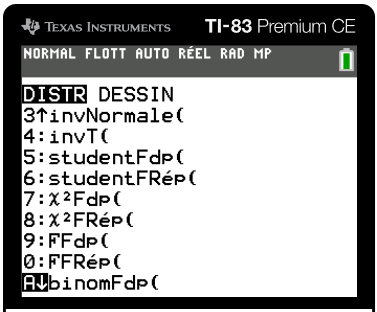
\includegraphics[width=0.27\linewidth]{ti01}\hfill 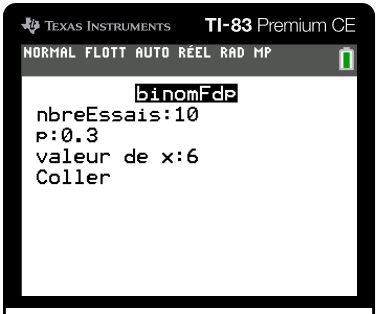
\includegraphics[width=0.27\linewidth]{ti02} \hfill 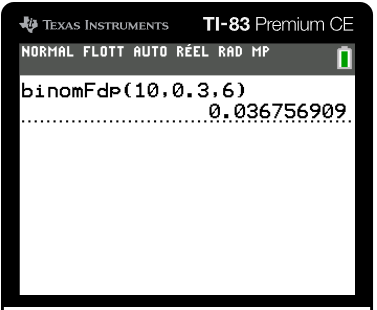
\includegraphics[width=0.27\linewidth]{ti03}

\textbf{Numworks} : Sélectionner \textbf{Probabilités} sur l'écran d'accueil, puis Binomiale. Entrer alors les valeurs des paramètres $n$ et $p$ puis valider.\\
Vous pouvez calculer des probabilités de la forme $\mathbb{P}(X\leqslant k)$, $\mathbb{P}(a\leqslant X \leqslant b)$, $\mathbb{P}(X \geqslant k)$ et $\mathbb{P}(X=k)$ en sélectionnant l'icône en haut à gauche de l'écran.

\vskip5pt

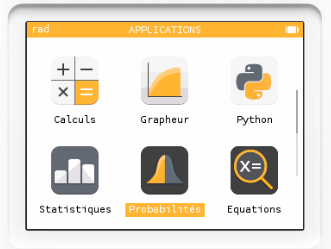
\includegraphics[width=0.23\linewidth]{num01}\hfill 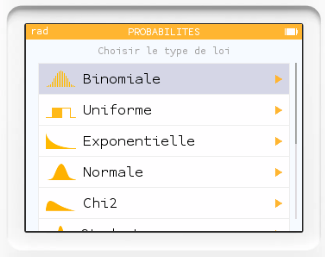
\includegraphics[width=0.23\linewidth]{num02}\hfill 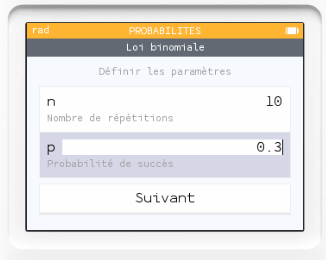
\includegraphics[width=0.23\linewidth]{num03} \hfill 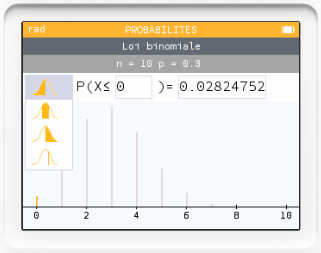
\includegraphics[width=0.23\linewidth]{num05}

\textbf{Casio Graph} : Dans le menu principal, sélectionner \textbf{STAT}. Appuyer ensuite sur \textbf{F5 [DIST]} puis \textbf{F5 [BINM]}.\\
Pour le calcul de $\mathbb{P}(X=k)$, appuyer sur \textbf{F1 [Bpd]}. Pour le calcul de $\mathbb{P}(X \leqslant k)$, appuyer sur \textbf{F2 [Bcd]}.\\
Sur l'écran suivant, placer le curseur sur \textbf{Data} et appuyer sur \textbf{F2 [Var]}. Renseigner alors les valeurs des paramètres de la loi binomiale et les valeurs de $k$.

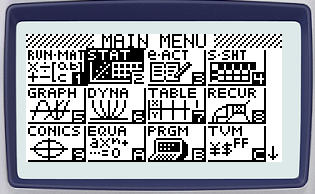
\includegraphics[width=0.23\linewidth]{casio01}\hfill 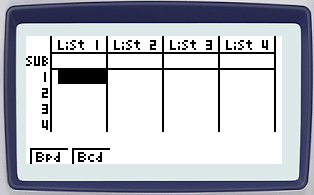
\includegraphics[width=0.23\linewidth]{casio04}\hfill 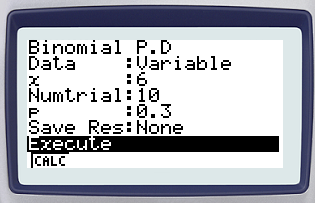
\includegraphics[width=0.23\linewidth]{casio05} \hfill 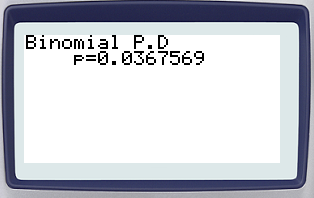
\includegraphics[width=0.23\linewidth]{casio06}


\subsubsection{Espérance, variance, écart-type}

\begin{proposition}Soit $X$ une variable aléatoire qui suit une loi binomiale $\mathcal{B}(n,p)$. L'espérance, la variance et l'écart-type de $X$ valent respectivement \[E[X]=np, \quad Var(X)=np(1-p), \quad \sigma(X)=\sqrt{np(1-p)}\]\end{proposition}

\begin{example}Un élève répond au hasard et de manière indépendante à un QCM de 20 questions. Chaque question laisse le choix entre 4 propositions dont une seule est correcte.

On note $X$ le nombre de bonnes réponses de l'élève. $X$ désigne donc le nombre de succès (bonnes réponses) d'un schéma de Bernoulli à 20 épreuves, chaque épreuve ayant une probabilité de succès de $\dfrac{1}{4}$. $X$ suit donc une loi binomiale $\mathcal{B}\left(20,\dfrac{1}{4}\right)$.

Ainsi, $E[X]=20 \times \dfrac{1}{4}=5$. L'élève peut espérer avoir 5 bonnes réponses.\end{example}


\chapter{Exercices}

\section*{Succession d'épreuves indépendantes}

\begin{exercise}On lance 3 fois un dé équilibré à 6 faces, numérotées de 1 à 6 et on regarde à chaque fois la face du dessus.
\begin{enumerate}
\item Quelle est la probabilité d'obtenir trois nombres pairs ?
\item Quelle est la probabilité d'obtenir un 6 au premier lancer mais de ne pas en obtenir au deuxième et troisième lancer ?
\end{enumerate}\end{exercise}

\begin{solution}À chaque lancer, on a une probabilité de $\dfrac{1}{2}$ d'obtenir un nombre pair. La probabilité d'obtenir 3 nombres pairs vaut donc $\dfrac{1}{2} \times \dfrac{1}{2} \times \dfrac{1}{2}= \dfrac{1}{8}$

La probabilité d'obtenir un 6 au premier lancer vaut $\dfrac{1}{6}$. La probabilité de ne pas obtenir 6 au deuxième lancer vaut $\dfrac{5}{6}$, et de même pour le troisième lancer. La probabilité recherchée est donc $\dfrac{1}{6} \times \dfrac{5}{6} \times \dfrac{5}{6}=\dfrac{25}{216}$
\end{solution}



\begin{exercise}Dix cartes sont placées sur la table, faces cachées : 2 piques, 4 carreaux et 4 trèfles. On sélectionne une carte au hasard, de manière uniforme. La carte est alors dévoilée et on note sa couleur. Puis elle est retournée et les cartes sont mélangées. On tire alors une autre carte et on regarde sa couleur. On notera $P$, $C$ et $T$ lorsque la carte choisie est respectivement un pique, un carreau ou un trèfle.
\begin{enumerate}
\item Construire l'arbre de probabilité de cette expérience. Combien a-t-on d'issues ?
\item Quelle est la probabilité de tirer deux trèfles ?
\item Quelle est la probabilité de tirer un pique puis un carreau ?
\item Quelle est la probabilité de ne pas tirer de trèfle ?
\item Quelle est la probabilité de tirer deux cartes de la même couleur ?
\end{enumerate}\end{exercise}

\begin{solution}

On peut construire l'arbre pondéré suivant

\tikzstyle{level 1}=[level distance=3.5cm, sibling distance=4cm]
\tikzstyle{level 2}=[level distance=3.5cm, sibling distance=1.5cm]
\tikzstyle{level 3}=[level distance=3.5cm, sibling distance=0.3cm]

% Define styles for bags and leafs
\tikzstyle{bag} = [text width=4em, text centered]
\tikzstyle{end} = [circle, minimum width=3pt,fill, inner sep=0pt]


\begin{center}
\begin{tikzpicture}[scale=0.8,grow=right,sloped]
\node[bag] { }
    child {
        node[bag] {T} 
        child {
                node[bag] {T}
                edge from parent node[below] {$0.4$}
            }
        child {
               node[bag] {C}
               edge from parent node[above] {$0.4$}
            }
        child {
                node[bag] {P}
                edge from parent node[above] {$0.2$}
            }
            edge from parent node[above] {$0.4$} 
    }
	child {
        node[bag] {C} 
        child {
                node[bag] {T}
                edge from parent node[below] {$0.4$}
            }
        child {
               node[bag] {C}
               edge from parent node[above] {$0.4$}
            }
        child {
                node[bag] {P}
                edge from parent node[above] {$0.2$}
            }
            edge from parent node[above] {$0.4$} 
    }
	child {
        node[bag] {P} 
        child {
                node[bag] {T}
                edge from parent node[below] {$0.4$}
            }
        child {
               node[bag] {C}
               edge from parent node[above] {$0.4$}
            }
        child {
                node[bag] {P}
                edge from parent node[above] {$0.2$}
            }
            edge from parent node[above] {$0.2$} 
    };
\end{tikzpicture}
\end{center}
La probabilité de tirer deux trèfles vaut $0,4 \times 0,4 = 0,16$.

La probabilité de tirer un pique puis un carreau vaut $0,2 \times 0,4 = 0,08$.

La probabilité de ne pas tirer de trèfle vaut $0,6 \times 0,6 = 0,36$.

La probabilité de tirer deux piques vaut $0,2 \times 0,2 = 0,04$. Celle de tirer deux carreaux vaut $0,4 \times 0,4 = 0,16$ et celle de tirer deux trèfles vaut aussi $0,16$. Finalement, la probabilité de tirer deux cartes de la même couleur veut $0,16+0,16+0,04=0,36$

\end{solution}




\begin{exercise}Une urne renferme deux boules rouges, trois boules bleues et cinq boules jaunes indiscernables au toucher. On tire successivement et avec remise trois boules dans l'urne
\begin{enumerate}
\item Quelle hypothèse permet d'affirmer que les tirages sont indépendants ?
\item Quelle est la probabilité de tirer 3 boules jaunes ?
\item Quelle est la probabilité de tirer une boule rouge puis deux boules bleues ?
\item Quelle est la probabilité de tirer 3 boules de couleur différente ?
\end{enumerate}\end{exercise}

\begin{solution}Le fait de remettre la boule tirée dans l'urne permet d'affirmer que les tirages sont indépendants

La probabilité de tirer 3 boules jaunes, c'est-à-dire la probabilité du triplet $(J;J;J)$ est de $\dfrac{1}{2} \times \dfrac{1}{2} \times \dfrac{1}{2}=\dfrac{1}{8}$

La probabilité de tirer une boule rouge puis deux boules bleues, c'est à-dire la probabilité du triplet $(R;B;B)$ vaut $\dfrac{1}{5} \times \dfrac{3}{10} \times \dfrac{3}{10}=\dfrac{9}{500}$

Les issues ayant 3 boules de couleurs différentes sont $(J;B;R)$, $(J;R;B)$, $(B;R;J)$, $(B;J;R)$, $(R;B;J)$ et $(R;J;B)$. Elles sont au nombre de 6, sont naturellement disjointes, et ont toutes les trois la même probabilité, à savoir $\dfrac{3}{10} \times 	\dfrac{1}{5} \times \dfrac{1}{2} = \dfrac{3}{100}$. La probabilité de tirer trois boules de couleur différente vaut donc $6 \times \dfrac{3}{100} = \dfrac{9}{50}$\end{solution}




\begin{exercise}Au dernier examen d'une université, composé de trois exercices, 70\% des élèves ont réussi l'exercice 1, 50\% ont réussi le deuxième et 25\% ont réussi le troisième. On suppose que la réussite d'un exercice est indépendante de la réussite de tous les autres. On interroge un étudiant uniformément au hasard.
\begin{enumerate}
\item Quelle est la probabilité que cet étudiant ait réussi les trois exercices ?
\item Quelle est la probabilité qu'il n'en ait réussi aucun ?
\item Quelle est la probabilité qu'il ait réussi exactement un exercice ?
\end{enumerate}\end{exercise}

\begin{solution}La probabilité que cet étudiant ait réussi les trois exercices vaut $0.7  \times 0.5 \times 0.25 = 0.0875$

La probabilité qu'il n'en ait réussi aucun vaut $(1-0.7)\times(1-0.5) \times (1-0.25)=0.1125$

La probabilité qu'il ait seulement réussi l'exercice 1 vaut $0.7 \times (1-0.5) \times (1-0.25)=0.2525$. La probabilité qu'il ait seulement réussi l'exercice 2 vaut $(1-0.7) \times 0.5 \times (1-0.25)=0.1125$.  La probabilité qu'il ait seulement réussi l'exercice 3 vaut $(1-0.7) \times (1-0.5) \times 0.25=0.0375$ La probabilité qu'il ait réussi exactement un exercice vaut donc $0.2625+0.1125+0.0375=0.4125$. \end{solution}




\begin{exercise}On lance $n$ fois un dé équilibré à 6 faces, numérotées de 1 à 6, puis on regarde à chaque fois la face du dessus. On note $A_n$ l'événement « le nombre 6 a été obtenu au moins une fois ».
\begin{enumerate}
\item Décrire l'événement $\overline{A_n}$ à l'aide d'une phrase puis déterminer $\mathbb{P}(\overline{A_n})$ et $\mathbb{P}(A_n)$. 
\item Quelle est la limite de $\mathbb{P}(A_n)$ ? Interpréter cette limite dans le contexte de l'exercice.
\item Combien de lancers faut-il effectuer pour être sûr à au moins 95\% que l'on obtiendra au moins une fois le nombre 6 en $n$ lancers ?
\end{enumerate}\end{exercise}


\begin{solution}$\overline{A_n}$ est l'événement « le nombre de 6 n'a été obtenu aucune fois ». Chaque lancer étant indépendant, sa probabilité vaut $\left(\dfrac{5}{6}\right)^n$. Ainsi, 
$\mathbb{P}(A_n)=1-\left(\dfrac{5}{6}\right)^n$.

Puisque $-1< \dfrac{5}{6} < 1$, on a $\displaystyle\lim_{n \to +\infty} \left(\dfrac{5}{6}\right)^n=0$ et donc $\displaystyle\lim_{n \to +\infty}\mathbb{P}(A_n)=1$. en lançant le dé un grand nombre de fois, on est quasiment certain d'obtenir au moins une fois le nombre 6.

Cherchons les entiers $n$ tels que $=1-\left(\dfrac{5}{6}\right)^n \geqslant 0.95$. On a alors $-\left(\dfrac{5}{6}\right)^n \geqslant -0.05$ et donc $\left(\dfrac{5}{6}\right)^n \leqslant 0.05$. On applique alors le logarithme népérien, qui est croissant sur $]0;+\infty[$, et on a donc $n \ln \left(\dfrac{5}{6}\right) \leqslant \ln(0.05)$. \\En divisant par $\ln\left(\dfrac{5}{6}\right)$ qui est négatif, on aboutit alors à $n \geqslant \dfrac{\ln(0.05)}{\ln\left(\frac{5}{6}\right)}\simeq 16.4$. \\En lançant 17 fois le dé, on a plus de 95\% de chances d'obtenir au moins une fois le nombre 6.\end{solution}





\begin{exercise}Un lycée présente $n$ candidats au recrutement dans une école, où $n$ est un entier naturel non nul.
On admet que la probabilité pour un candidat quelconque du lycée d'être admis à l'école
est égale à $0,24$ et que les résultats des candidats sont indépendants les uns des autres.
\begin{enumerate}
\item Donner l'expression, en fonction de $n$, de la probabilité qu'aucun candidat issu de ce
lycée ne soit admis à l'école.
\item À partir de quelle valeur de l'entier $n$ la probabilité qu'au moins un élève de ce lycée
soit admis à l'école est-elle supérieure ou égale à 0,99 ?\end{enumerate}\end{exercise}

\begin{solution}La probabilité qu'aucun élève ne soit admis vaut $0.76^n$.

La probabilité qu'au moins un élève soit admis vaut donc $1-0.76^n$. Or, $1-0.76^n \geqslant 0.99$ si et seulement si $-0.76^n \geqslant -0.01$ soit $0.76^n \leqslant 0.01$. On applique alors le logarithme népérien, qui est croissant sur $]0;+\infty[$, et on a donc $n \ln(0.76) \leqslant \ln(0.01)$. \\ En divisant par $\ln\left(0.76\right)$ qui est négatif, on aboutit alors à $n \geqslant \dfrac{\ln(0.01)}{\ln(0.76)}\simeq 16.8$. A partir de 17 candidats, la probabilité qu'un élève du lycée soit admis dans cette école est supérieure à 99\%.\end{solution}




\section*{Loi binomiale}


%
%\begin{exercise}Donner les valeurs de $\dbinom{5}{3}$, $\dbinom{7}{5}$, $\dbinom{10}{7}$,  $\dbinom{8}{4}$, $\dbinom{10}{4}$ et $\dbinom{7}{3}$.\end{exercise}
%
%\begin{solution}\hspace{0pt}
%\begin{itemize}
%\item $\dbinom{5}{3}=\dfrac{5!}{3!2!}=\dfrac{120}{6 \times 2}=10$
%\item $\dbinom{7}{5}=\dfrac{7!}{5!2!}=\dfrac{7 \times 6 \times 5!}{5! \times 2}= \dfrac{7 \times 6}{2}=21$
%\item $\dbinom{10}{7}=\dfrac{10!}{7!3!}=\dfrac{10 \times 9 \times 8 \times 7!}{7! \times 3!}=\dfrac{10 \times 9 \times 8}{6}=120$
%\item $\dbinom{8}{4}=\dfrac{8!}{4!4!}=\dfrac{8 \times 7 \times 6 \times 5 \times 4!}{4! \times 4!}=\dfrac{8 \times 7 \times 6 \times 5}{4 \times 3 \times 2 \times 1}=70$
%\item $\dbinom{10}{4}=\dfrac{10!}{4!6!}=\dfrac{10 \times 9 \times 8 \times 7 \times 6!}{4! \times 6!}=\dfrac{10 \times 9 \times 8 \times 7}{4 \times 3 \times 2 \times 1}=210$
%\item $\dbinom{7}{3}=\dfrac{7!}{3!4!}=\dfrac{7 \times 6 \times 5 \times 4!}{3! \times 4!}=35$
%\end{itemize}\end{solution}
%
%
%
%\begin{exercise}Calculer les coefficients binomiaux : $\dbinom{51}{2}$, $\dbinom{1475}{1474}$, $\dbinom{1321}{0}$, $\dbinom{26}{24}$\end{exercise}
%
%\begin{solution} $\dbinom{51}{2} = \dfrac{51 \times 50}{2}= 1275$, $\dbinom{1475}{1474}=\dbinom{1475}{1}=1475$, $\dbinom{1321}{0}=1$, $\dbinom{26}{24}=\dbinom{26}{2}=\dfrac{26 \times 25}{2}=325$\end{solution}

\begin{exercise}
Pour chacune des situations suivantes, dire si la variable aléatoire  suit ou non une loi binomiale. Si c'est le cas, préciser ses paramètres.

\begin{enumerate}
\item On lance trois fois une pièce de monnaie équilibrée et on note $X$ le nombre de fois où la pièce où l'on obtient PILE.
\item On lance simultanément 5 dés équilibrés à 6 faces, numérotées de 1 à 6 ainsi que 3 dés équilibrés à 4 faces, numérotées de 1 à 4. On note $X$ le nombre de faces 3 obtenues.
\item On lance simultanément 5 dés équilibrés à 6 faces, numérotées de 1 à 6 ainsi que 3 dés équilibrés à 4 faces, numérotées de 1 à 4. On note $X$ le nombre de faces 5 obtenues.
\item D'après un sondage, 65\% des Français se rendent au restaurant au moins une fois par mois. On interroge 30 Français au hasard et on note $X$ le nombre de Français qui vont au restaurant au moins une fois par mois dans cet échantillon. On suppose que ce tirage peut être assimilé à un tirage avec remise.
\item Un élève répond au hasard à un QCM composé de 20 questions. Pour chaque question, une seule réponse est correcte et l'élève en choisit une au hasard, indépendamment de ses autres réponses. On note $X$ le nombre de réponses correctes à l'issue du questionnaire.
\item Un élève répond au hasard à un QCM composé de 20 questions. Pour chaque question, une seule réponse est correcte et l'élève en choisit une au hasard, indépendamment de ses autres réponses. Une réponse correcte rapporte 3 points, une réponse fausse en retire 1. On suppose que l'élève répond à toutes les questions et on note $X$ le nombre de points de cet élève à l'issue du questionnaire.
\item On répète 10 fois l'opération suivante : on lance simultanément 3 pièces de monnaie équilibrée. Sur ces 10 expériences, on note $X$ le nombre de fois où les 3 pièces de monnaie sont tombées du même côté.
\end{enumerate}
\end{exercise}

\begin{solution}\hspace{0pt}
\begin{enumerate}
\item $X$ compte le nombre de succès (obtenir Pile) après une succession de 3 lancers identiques indépendants. La probabilité de succès sur une épreuve est de $\dfrac{1}{2}$. La variable aléatoire $X$ suit une loi binomiale de paramètres $n=3$ et $p=\frac{1}{2}$.
\item Les expériences ne sont pas identiques : la probabilité d'obtenir un 3 sur un dé à 6 faces vaut $\frac{1}{6}$ alors que pour un dé à 4 faces, elle vaut $\frac{1}{4}$. $X$ ne suit donc pas une loi binomiale.
\item Il n'est pas possible d'obtenir 5 sur un dé à 4 faces, seuls les dés à 6 faces importent donc. On compte le nombre de succès après une succession de 5 lancers identiques et indépendants. $X$ suit donc une loi binomiale de paramètres $n=5$ et $p=\frac{1}{6}$.
\item Le tirage est assimilé à un tirage avec remise, ce qui suppose donc que les tirages sont indépendants. $X$ compte alors le nombre de succès (la personne tirée au hasard va au restaurant au moins une fois par mois) d'une répétition de 30 tirages. $X$ suit donc une loi binomiale de paramètres $n=30$ et $p=0,65$.
\item Les réponses étant données de manière identique et indépendante, $X$ suit donc une loi binomiale de paramètres $n=20$ et $p=\frac{1}{4}$.
\item Ici, $X$ ne compte pas le nombre de succès mais un nombre de points. $X$ ne suit donc pas une loi binomiale.
\item La probabilité que les pièces tombent sur la même face est de $\frac{1}{4}$. $X$ suit donc une loi binomiale de paramètres $n=10$ et $p=\frac{1}{4}$.
\end{enumerate}

\end{solution}


\begin{exercise}Soit $X$ une variable aléatoire suivant une loi binomiale $\mathcal{B}\left(5;\dfrac{1}{3}\right)$. Calculer $\mathbb{P}(X=1)$,  $\mathbb{P}(X \geqslant 4)$ et $\mathbb{P}(X<3)$\end{exercise}

\begin{solution}$\mathbb{P}(X=1)=\dbinom{5}{1} \times \dfrac{1}{3} \times \left(\dfrac{2}{3}\right)^4=5\times \dfrac{1}{3} \times \dfrac{16}{81}=\dfrac{80}{243}$

D'une part, $\mathbb{P}(X \geqslant 4)=\mathbb{P}(X=4) + \mathbb{P}(X=5)$. Or,
\begin{itemize}
\item $\mathbb{P}(X=4)=\dbinom{5}{4} \times \left(\dfrac{1}{3}\right)^4 \times \dfrac{2}{3}=5 \times \dfrac{1}{81} \times \dfrac{2}{3}=\dfrac{10}{243}$
\item $\mathbb{P}(X=5)=\dbinom{5}{5} \times \left( \dfrac{1}{3}\right)^5 \times \left(\dfrac{2}{3}\right)^0 = \dfrac{1}{243}$
\item Ainsi, $\mathbb{P}(X \geqslant 4)= \dfrac{11}{243}+\dfrac{1}{243}=\dfrac{12}{243}$
\end{itemize}

D'une part, $\mathbb{P}(X<3)=\mathbb{P}(X=0)+\mathbb{P}(X=1)+\mathbb{P}(X=2)$. Or,
\begin{itemize}
\item $\mathbb{P}(X=0)= \left(\dfrac{2}{3}\right)^5=\dfrac{32}{243}$
\item $\mathbb{P}(X=1)= \dfrac{80}{243}$ d'après la question 1
\item $\mathbb{P}(X=2)= \dbinom{5}{2} \times \left( \dfrac{1}{3}\right)^2 \times \left( \dfrac{2}{3} \right)^3 = \dfrac{5 \times 4}{2} \times \dfrac{1}{9} \times \dfrac{8}{27}=\dfrac{80}{243}$
\item Ainsi, $\mathbb{P}(X<3)=\dfrac{32}{243}+\dfrac{80}{243}+\dfrac{80}{243}=\dfrac{192}{243}=\dfrac{64}{81}$
\end{itemize}
\end{solution} 



\begin{exercise}[subtitle={(Amérique du Nord 2023)}]Soit $X$ une variable aléatoire suivant la loi binomiale $\mathcal{B}(3;p)$. On sait que $\mathbb{P}(X=0)=\dfrac{1}{125}$. Que vaut $p$ ?\end{exercise}

\begin{solution}On sait que $\mathbb{P}(X=0)=\dbinom{3}{0}p^0(1-p)^3=(1-p)^3=\dfrac{1}{125}$. Ainsi, $1-p=\dfrac{1}{5}$ et $p=\dfrac{4}{5}$.\end{solution}



%\begin{exercise}Soit $X$ une variable aléatoire suivant une loi binomiale $\mathcal{B}(4;0.25)$.
%\begin{enumerate}
%\item Résumer la loi de $X$ dans un tableau
%\item Calculer l'espérance de $X$. Nous verrons un peu plus tard une formule bien commode pour la déterminer.
%\end{enumerate}\end{exercise}
%
%\begin{solution}Le tableau résumant la loi de $X$ est le suivant
%
%\begin{tabularx}{\linewidth}{|X|X|X|X|X|X|}
%\hline
%$k$ & 0 & 1 & 2 & 3 & 4 \\
%\hline
%$\mathbb{P}(X=k)$ & $\dfrac{81}{256}$ & $\dfrac{27}{64}$ & $\dfrac{27}{128}$ & $\dfrac{3}{64}$ & $\dfrac{1}{256}$\\
%\hline
%\end{tabularx}
%
%A partir de ce tableau, on peut calculer l'espérance de $X$.
%\[ \mathbb{E}(X)= 0 \times \dfrac{81}{256} + 1 \times \dfrac{27}{64} + 2 \times \dfrac{27}{128}+ 3 \times \dfrac{3}{64}+ 4 \times \dfrac{1}{256}=1\]
%\end{solution}




\begin{exercise}On lance 4 fois un dé équilibré à 6 faces, numérotées de 1 à 6. 
\begin{enumerate}
\item On note $X$ la variable aléatoire qui compte le nombre de 3 obtenus. Quelle est la loi de $X$ ?
\item Que valent $\mathbb{P}(X=1)$ et $\mathbb{P}(X \leqslant 3)$ ?
\end{enumerate} \newpage \end{exercise}

\begin{solution}$X$ suit une loi binomiale de paramètres $4$ et $\dfrac{1}{6}$. 

On a $\mathbb{P}(X=1)=\dbinom{4}{1} \left(\dfrac{1}{6}\right)^1 \left(1-\dfrac{1}{6}\right)^{4-1}=\dfrac{125}{324}$

On peut calculer pour toutes les issues qui vérifient $X\leqslant3$ : 
\[\mathbb{P}(X \leqslant 3) = \mathbb{P}(X=0)+\mathbb{P}(X=1)+\mathbb{P}(X=2)+\mathbb{P}(X=3)\] 
Or,
\begin{itemize}
\item $\mathbb{P}(X=0)=\left(\dfrac{5}{6}\right)^4=\dfrac{625}{1296}$
\item $\mathbb{P}(X=1)=\dfrac{125}{324}=\dfrac{500}{1296}$
\item $\mathbb{P}(X=2)= \dbinom{4}{2} \left(\dfrac{1}{6}\right)^2 \left(\dfrac{5}{6}\right)^2= \dfrac{150}{1296}$
\item $\mathbb{P}(X=3)= \dbinom{4}{3} \left(\dfrac{1}{6}\right)^3 \left(\dfrac{5}{6}\right)^1= \dfrac{20}{1296}$
\end{itemize}
Ainsi, $\mathbb{P}(X \leqslant 3)=\dfrac{1295}{1296}$. Il est aussi possible (et plus facile) de calculer la probabilité de l'événement complémentaire $X>3$. Celui-ci est composé d'une seule issue.
\[ \mathbb{P}(X>3)=\mathbb{P}(X=4)= \dbinom{4}{4} \left( \dfrac{1}{6}\right)^4 \left( \dfrac{5}{6}\right)^0=\dfrac{1}{1296}\]
Ainsi, 
\[ \mathbb{P}(X\leqslant 3)=1- \mathbb{P}(X>3)=1-\dfrac{1}{1296}=\dfrac{1295}{1296}\]\end{solution}


\begin{exercise}[subtitle={(Amérique du Nord 2024)}]Dans cet exercice, les probabilités seront arrondies au dis-millième.

On choisit 500 véhicules particuliers hybrides rechargeables immatriculés en France en 2022. On admettra que la probabilité qu'un tel véhicule soit neuf est égale à 0,65.
On assimile le choix de ces 500 véhicules à un tirage aléatoire avec remise.

On appelle $X$ la variable aléatoire représentant le nombre de véhicules neufs parmi les 500 véhicules choisis.
\begin{enumerate}
\item On admet que la variable aléatoire $X$ suit une loi binomiale. Préciser la valeur de ses paramètres.
\item Déterminer la probabilité qu'exactement 325 de ces véhicules soient neufs.
\item Déterminer la probabilité $\mathbb{P}(X \geqslant 325)$ puis interpréter le résultat dans le contexte de l'exercice.\end{enumerate}

\end{exercise}

\begin{solution}La variable aléatoire $X$ suit une loi binomiale de paramètres $n=500$ et $p=0,65$. En utilisant la calculatrice, on trouve $\mathbb{P}(X=325) \simeq 0,0374$ et $\mathbb{P}(X \geqslant 325)\simeq 0,5206$.\end{solution}

\begin{exercise}

Une entreprise produit des composants électroniques, dont on estime que 5\% d'entre eux sont défectueux. On prélève 10 composants parmi le stock. On suppose que le stock est assez grand pour que cette sélection soit assimilée à un tirage avec remise dans le stock. On note $X$ le nombre de composants défectueux ainsi piochés.

\begin{enumerate}
\item Quelle est la loi de la variable aléatoire $X$ ?
\item Quelle est la probabilité qu'aucune pièce ne soit défectueuse ?
\item Que vaut $\mathbb{P}(X \leqslant 2)$ ? 
\item Combien de composants doit-on prélever pour être sûr à au moins 99\% de piocher au moins un composant défectueux dans ce lot ?
\end{enumerate}\end{exercise}

\begin{solution}
La variable aléatoire $X$ suit une loi binomiale de paramètres 10 et 0,05.

La probabilité qu'aucune pièce ne soit défectueuse correspond à $\mathbb{P}(X=0)$. $\mathbb{P}(X=0)= 0.95^{10} \simeq 0.599$.

On a $\mathbb{P}(X \leqslant 2) = \mathbb{P}(X =0) + \mathbb{P}(X=1)  + \mathbb{P}(X=2)$. Or,
\begin{itemize}
\item $\mathbb{P}(X=0)=0.95^{10}$
\item $\mathbb{P}(X=1)=10 \times 0.05 \times 0.95 ^9 = 0.5 \times 0.95 ^9$
\item $\mathbb{P}(X=2)= 45 \times 0.05^2 \times 0.95^8 = 0.1125 \times 0.9^8$
\item Finalement $\mathbb{P}(X \leqslant 2)= 0.95^{10}+0.5 \times 0.95^9 + 0.1125 \times 0.9^8 \simeq 0.988$
\end{itemize} Il y a environ 98,8 \% de chances que le nombre de pièces défectueuses soit inférieur ou égal à 2.

Soit $n$ le nombre de composants prélevés et $Y$ le nombre de composants défectueux obtenus. \\On a $\mathbb{P}(Y\geqslant 1)=1-\mathbb{P}(Y=0)=1-0.95^n$. Or, $1-0.95^n \geqslant 0.99$ ssi $0.95^n \leqslant 0.01$. En appliquant le logarithme népérien, qui est croissant sur $]0:+\infty[$, on obtient alors $n \ln(0.95) \leqslant \ln(0.01)$ puis en divisant par $\ln(0.95)$, qui est négatif, on aboutit à $n \geqslant \dfrac{\ln(0.01)}{\ln(0.95)}\simeq 89.8$. Il faut donc prélever 90 pièces pour être sûr à au moins 99\% d'en avoir au moins une défectueuse.
\end{solution}


\begin{exercise}
On lance quatre fois une pièce équilibrée et on regarde sur quel côté elle tombe. On note $X$ la variable aléatoire qui compte le nombre de PILE
\begin{enumerate}
\item Quelle est la loi de $X$ ?
\item Quel est la probabilité de ne tomber aucune fois sur PILE ?
\item Quelle est la probabilité d'obtenir exactement 2 PILE ?
\item Quelle est la probabilité d'obtenir au plus 2 PILE ?
\item En moyenne, combien obtiendra-t-on de PILE ?
\item Reprendre les questions précédentes en lançant 5 fois une pièce truquée dont la probabilité de tomber sur PILE vaut 0.6.
\end{enumerate}\end{exercise}

\begin{solution}$X$ suit une loi binomiale de paramètres 4 et $\dfrac{1}{2}$. 

La probabilité de ne tomber aucune fois sur PILE correspond à $\mathbb{P}(X=0)$, $\mathbb{P}(X=0)= \left(	\dfrac{1}{2}\right)^4 = \dfrac{1}{16}$

La probabilité d'obtenir exactement 2 PILE correspond à $\mathbb{P}(X=2)$
\[ \mathbb{P}(X=2) = \dbinom{4}{2} \left( \dfrac{1}{2}\right)^2 \left( \dfrac{1}{2}\right)^2=6 \times  \dfrac{1}{4} \times \dfrac{1}{4}=\dfrac{3}{8}\]

 La probabilité d'obtenir au plus 2 PILE correspond à $\mathbb{P}(X \leqslant 2)$, soit $\mathbb{P}(X=0)+\mathbb{P}(X=1)+\mathbb{P}(X=2)$. Il reste à calculer $\mathbb{P}(X=1)$
\begin{itemize}
\item $\mathbb{P}(X=1)= \dbinom{4}{1} \times \dfrac{1}{2} \times \dfrac{1}{2^3}=\dfrac{3}{8}$
\item Ainsi, $\mathbb{P}(X \leqslant 2)=\dfrac{1}{16}+\dfrac{3}{8}+\dfrac{3}{8}=\dfrac{13}{16}$
\end{itemize}

On a $E[X]=4 \times 0.5=2$. En moyenne, on obtient 2 PILE.

Si maintenant on lance 5 fois une pièce truquée dont la probabilité de tomber sur PILE vaut 0.6. Notons $Y$ la variable aléatoire qui compte le nombre de PILE obtenus. $Y$ suit une loi binomiale de paramètres 5 et 0.6. 

On a alors $\mathbb{P}(Y=0)=0.4^5=0.01024$, $\mathbb{P}(Y=2)= \dbinom{5}{2} \times 0.6^2\times 0.4^3=0.2304$.

Par ailleurs, $\mathbb{P}(Y=1)=\dbinom{5}{1} \times 0.6^1 \times 0.4^4 =0.0768$. \\Ainsi, $\mathbb{P}(Y \leqslant 2)=0.01024 + 0.0768+0.2304 =0.31744$.

Enfin, $E[Y]=5 \times 0.6 = 3$. En moyenne, on obtiendra 3 PILE. 
\end{solution}




\begin{exercise}Dans cet exercice, les probabilités calculées seront arrondies, si nécessaire, à $10^{-3}$ près.

Une entreprise produit des stylos en grande quantité. La probabilité qu'un stylo présente un défaut est de $0,1$.


On prélève 10 stylos dans le stock de cet entreprise. On suppose que le nombre de stylos produits est suffisamment grand pour que cette sélection soit assimilée à des tirages indépendants et avec remise. On note $X$ le nombre de stylos défectueux ainsi piochés.
\begin{enumerate}
\item Quelle est la loi de $X$ ? On précisera ses paramètres.
\item Donner l'espérance et la variance de $X$.
\item Calculer la probabilité qu'il y ait exactement un stylo défectueux.
\item Calculer la probabilité qu'il y ait au moins un stylo défectueux.
\item Calculer la probabilité qu'il y ait au plus deux stylos défectueux.
\end{enumerate}\newpage \end{exercise}

\begin{solution}\hspace{0pt}
\begin{enumerate}
\item $X$ suit une loi binomiale de paramètres 10 et 0.1.
\item On a $E(X)=10 \times 0.1 = 1$ et $Var(X)=10 \times 0.1 \times (1-0.1)=0.9$.
\item On a a $\mathbb{P}(X=1)=\dbinom{10}{1} \times 0.1^1 \times 0.9 ^9 \simeq 0.387$.
\item On a $\mathbb{P}(X \geqslant 1)=1-\mathbb{P}(X=0)=1-0.9^{10}\simeq 0.651$
\item  On a $\mathbb{P}(X\leqslant 2)=\mathbb{P}(X=0) + \mathbb{P}(X=1) + \mathbb{P}(X=2)$

Ainsi, $\mathbb{P}(X\leqslant 2) = 0.9^{10}+\dbinom{10}{1} \times 0.1^1 \times 0.9 ^9  + \dbinom{10}{2} \times 0.1^2 \times 0.9 ^98 \simeq 0.930$
\end{enumerate}\end{solution}


\begin{exercise}[subtitle={(Asie 2024)}]
Dans la revue \textit{Lancet Public Health}, les chercheurs affirment qu’au 11 mai 2020, 5,7\% des adultes français avaient déjà été infectés par la COVID 19.

\begin{enumerate}
\item On prélève un individu dans la population française adulte au 11 mai 2020.\\
On note I l'évènement : « l'adulte a déjà été infecté par la COVID 19 »\\
Quelle est la probabilité que cet individu prélevé ait déjà été infecté par la COVID 19 ?
\item On prélève un échantillon de 100 personnes de la population supposées choisies de façon indépendante les unes des autres.\\ On assimile ce prélèvement à un tirage avec remise. \\On appelle $X$ la variable aléatoire qui compte le nombre de personnes ayant déjà été infectées.
\begin{enumerate}
\item Justifier que $X$ suit une loi binomiale dont on donnera les paramètres.
\item Calculer son espérance mathématique. Interpréter ce résultat dans le cadre
de l'exercice.
\item Quelle est la probabilité qu'il n'y ait aucune personne infectée dans l'échantillon ?
On donnera une valeur approchée à $10^{-4}$ près du résultat.
\item Quelle est la probabilité qu'il y ait au moins 2 personnes infectées dans l'échantillon ?
On donnera une valeur approchée à $10^{-4}$ près du résultat.
\item Déterminer le plus petit entier $n$ tel que $\mathbb{P}(X \leqslant n) \geqslant 0,9$.
Interpréter ce résultat dans le contexte de l'exercice.\end{enumerate}
\end{enumerate}
\end{exercise}

\begin{solution}\hspace{0pt}
\begin{enumerate}
\item On a $\mathbb{P}(I)=0,057$.
\item \begin{enumerate}
\item Le prélèvement est assimilé à un tirage avec remise, ce qui signifie que les personnes sélectionnées le sont de manière identique et indépendante. $X$ compte le nombre de succès d'un schéma de Bernoulli à 100 épreuves, de probabilité de succès 0,057. $X$ suit donc une loi binomiale de paramètres $n=100$ et $p=0,057$.
\item On a $E[X]=100 \times 0,057=5,7$. Sur un échantillon de 100 personnes, en moyenne 5,7 d'entre elles ont déjà été infectées par la COVID 19.
\item On a $\mathbb{P}(X=0)=\dbinom{100}{0} \times 0,057^0 \times (1-0,057)^0 \simeq 0,0028$.
\item On a $\mathbb{P}(X \geqslant 2) \simeq 0,9801$.
\item On trouve $\mathbb{P}(X \leqslant 8) \simeq 0,8829$ et $\mathbb{P}(X \leqslant 9) \simeq 0,9408$. L'entier recherché est donc 9. Cela signifie que sur un échantillon de 100 personnes, la probabilité qu'au plus 9 d'entre elles aient déjà été infectées par la COVID 19 est supérieure à 0,9.
\end{enumerate}
\end{enumerate}

\end{solution}


\begin{exercise}[subtitle={(Asie 2015)}]
Un concurrent participe à un concours de tir à l'arc, sur une cible circulaire. A chaque tir, la probabilité qu'il atteigne la cible est égale à $0,8$.
\begin{enumerate}
\item Le concurrent tire quatre flèches. On considère que les tirs sont indépendants. Déterminer la probabilité qu'il atteigne au moins trois fois la cible.
\item Combien de flèches le concurrent doit-il prévoir pour atteindre en moyenne la cible 12 fois ?
\end{enumerate} 
 \end{exercise}
 
 \begin{solution}
Soit $X$ la variable aléatoire qui compte le nombre de flèches qui atteignent la cible en 4 tirs. Les tirs étant indépendants, $X$ suit une loi binomiale de paramètres 4 et 0.8. Ainsi, $\mathbb{P}(X=3)=\dbinom{4}{3}0.8^3 \times 0.2^1 = 0.4096$.

Soit $n$ un entier naturel et $Y$ la variable aléatoire qui compte le nombre de flèches qui atteignent la cible en $n$ tirs. Les tirs étant indépendants, $Y$ suit une loi binomiale de paramètres $n$ et 0.8. Par ailleurs, $E(Y)=0.8n$. Ainsi, $E(Y)=12$ si $n=15$. Il lui faut 15 flèches pour espérer atteindre la cible 12 fois.
\end{solution}

\begin{exercise}
Soit $X$ une variable aléatoire suivant une loi binomiale de paramètres $n$ et $p$. On suppose que $E[X]=3,36$ et $\sigma(X)=1,68$.

Calculer $\pp (2\leqslant X \leqslant 5)$. On donnera une réponse arrondie au dix-millième.
\end{exercise}

\begin{solution}
On sait que $E[X]=np=3,36$ et $V(X)=\sigma(X)^2=2,8224=np(1-p)=3,36 \times(1-p)$. Ainsi, $1-p=\dfrac{2,8824}{3,36}=0,84$ et donc $p=0,16$.

Ainsi, on a $np=3,36$ soit $n=\dfrac{3,36}{0,16}=21$.

$X$ suit donc une loi binomiale de paramètres $n=21$ et $p=0,84$. On trouve alors $\mathbb{P}(2\leqslant X \leqslant 5) \simeq 0,7655$.
\end{solution}


\begin{exercise}
Une urne contient un très grand nombre de boules rouges et de boules noires, indiscernables au toucher. On note $p$ la proportion de boules rouges dans cette urne. On tire 20 fois, et avec remise, une boule dans cette urne et on note $X$ le nombre de boules rouges obtenues.

\begin{enumerate}
\item Quelle est la loi de la variable aléatoire $X$ ?
\end{enumerate}
On effectue un tel tirage et on obtient alors 5 boules rouges. À partir de cette information, on souhaite déterminer le nombre de boules rouges dans l'urne en utilisant la méthode du maximum de vraisemblance : cette méthode consiste à déterminer la valeur de la proportion $p$ pour laquelle la probabilité $\mathbb{P}(X=5)$ est maximale.

\begin{enumerate}
\setcounter{enumi}{1}
\item Exprimer $\mathbb{P}(X=5)$ en fonction de $p$.

\item Pour tout réel $x\in[0;1]$, on note $f(x)=x^5(1-x)^{15}$. On admet que la fonction $f$ ainsi définie est dérivable sur $[0;1]$.
\begin{enumerate}
\item  Montrer que, pour tout réel $x$, on a $f'(x)=-5x^4(4x-1)(1-x)^{14}$.     
\item En déduire que $f$ admet un maximum sur $[0;1]$ en une valeur que l'on précisera.
\end{enumerate}
\item Conclure à l'aide des résultats précédents.
\end{enumerate}
\newpage
\end{exercise}

\begin{solution}\hspace{0pt}
\begin{enumerate}
\item La variable aléatoire $X$ suit une loi binomiale de paramètres $n=20$ et $p$.
\item On a $\mathbb{P}(X=5)=\dbinom{20}{5} \times p^5 \times (1-p)^{15}$.
\item 
\begin{enumerate}
\item Pour tout réel $x\in [0;1]$, on a $f'(x)=5x^4 \times (1-x)^{15}+x^5\times (-15)(1-x)^{14}=5x^4 \times (1-x)^{14} \times ((1-x)-3x)$. Finalement, on a $f'(x)=-5x^4(4x-1)(1-x)^{14}$.
\item Pour tout réel $x\in [0;1]$, on a $-5x^4 \leqslant 0$ et $(1-x)^{14}\geqslant 0$. $f'(x)$ est donc du signe opposé à $4x-1$.

\begin{center}
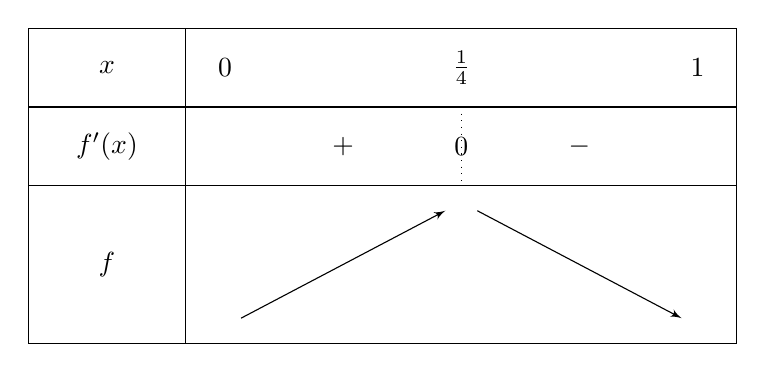
\begin{tikzpicture}[scale=1]
   \tkzTabInit{$x$ / 1 ,$f'(x)$/1,$f$/2}{$0$, $\frac{1}{4}$, $1$}
      \tkzTabLine{, +, z, -,  }
   \tkzTabVar{-/$ $,+/$ $,-/$ $}
\end{tikzpicture}
\end{center}

La fonction $f$ admet un maximum sur $[0;1]$ en $\dfrac{1}{4}$.

\end{enumerate}
\item On remarque que $\mathbb{P}(X=5)= \dbinom{20}{5}f(p)$. Cette probabilité est donc maximale lorsque $f$ est maximale, c'est-à-dire pour $p=\dfrac{1}{4}$. La méthode d'estimation par maximum de vraisemblance nous indique donc que la proportion de boules rouges dans l'urne est de $\dfrac{1}{4}$.
\end{enumerate}
\end{solution}


%\begin{exercise}Un examinateur fait passer des étudiants à un oral. Il possède 40 exercices différents, dont 3 concernent les probabilités. Pour chaque étudiant, l'examinateur choisit au hasard un de ses 40 sujets et ce, indépendamment des sujets précédemment tirés.
%\begin{enumerate}
%\item La matinée de l'examinateur comporte 5 étudiants à faire passer. Quelle est la probabilité qu'un sujet de probabilité tombe au moins une fois durant cette matinée ?
%\item Combien d'élèves l'examinateur doit-il interroger pour qu'en moyenne 6 élèves soient interrogés sur un sujet de probabilité ?
%\item Combien d'élèves l'examinateur doit-il faire passer pour avoir au moins 95\% de chance qu'un sujet de probabilité soit tiré au cours de cette session ?
%\item L'examinateur fait passer $n$ étudiants. On note $A$ l'événement « au moins deux étudiants sont tombés sur un sujet de probabilités ».
%\begin{enumerate}
%\item Justifier que $\mathbb{P}(A)=1- \left( \dfrac{37}{40}\right)^{n}-\dfrac{3n}{40} \times \left( \dfrac{37}{40}\right)^{n-1}$
%\item Combien d'élèves l'examinateur doit-il interroger pour avoir au moins 70\% de chances qu'au moins deux étudiants tombent sur un sujet de probabilités ? (ne pas résoudre directement l'inéquation, procéder par exemple à l'aide d'un algorithme).
%\end{enumerate}
%\end{enumerate}\end{exercise}


%\begin{solution}\hspace{0pt}
%\begin{enumerate}
%\item Notons $X$ le nombre de sujet de probabilités tombés durant cette matinée. $X$ suit une loi binomiale de paramètres 5 et $\dfrac{3}{40}$. Ainsi, $\mathbb{P}(X\geqslant 1)=1-\mathbb{P}(X=0)=1-\left(\dfrac{37}{40}\right)^5\simeq 0.323$
%\item Soit $n$ un entier naturel et $Y$ la variable aléatoire qui donne le nombre d'élèves tombés sur un sujet de probabilités; $Y$ suit une loi binomiale de paramètres $n$ et $\dfrac{3}{40}$. Par ailleurs, $E(Y)=\dfrac{3n}{40}$. Ainsi, $E(Y)=6$ ssi $n=80$. L'examinateur doit interroger 80 élèves pour qu'en moyenne 6 élèves soient interrogés sur un sujet de probabilité.
%\item On a $\mathbb{P}(Y \geqslant 1)=1-\mathbb{P}(Y=0)=1-\left(\dfrac{37}{40}\right)^n$. Or, $1-\left(\dfrac{37}{40}\right)^n \geqslant 0.95$ si et seulement si $\left(\dfrac{37}{40}\right)^n\leqslant 0.05$ soit, par croissance de $\ln$ sur $]0;+\infty[$, $n \ln \dfrac{37}{40} \leqslant \ln(0.05)$ et donc $n \geqslant \dfrac{\ln(0.05)}{\ln \frac{37}{40}}\simeq 38.42$. L'examinateur doit interroger au moins 39 élèves pour avoir au moins 95\% de chance qu'un sujet de probabilité soit tiré au cours de cette session.
%\item
%\begin{enumerate}
%\item On a $\mathbb{P}(Y\geqslant 2)=1-\mathbb{P}(Y<2)=1-(\mathbb{P}(Y=0)+\mathbb{P}(Y=1))$. Or, $\mathbb{P}(Y=0)=\left(\dfrac{37}{40}\right)^n$ et $\mathbb{P}(Y=1)=\dbinom{n}{1}\dfrac{3}{40} \times \left(\dfrac{37}{40}\right)^{n-1}=\left( \dfrac{37}{40}\right)^{n-1}$. Ainsi, $\mathbb{P}(A)=1- \left( \dfrac{37}{40}\right)^{n}-\dfrac{3n}{40} \times \left( \dfrac{37}{40}\right)^{n-1}$
%\item A l'aide de la calculatrice, on trouve que l'examinateur doit interroger 32 élèves pour avoir au moins 70\% de chances qu'au moins deux étudiants tombent sur un sujet de probabilités .
%\end{enumerate}
%\end{enumerate}
%
%\end{solution}


\section*{Exercices de synthèse}




\begin{exercise}[subtitle={(Réunion 2023)}]
Un commerçant vend deux types de matelas : matelas RESSORTS et matelas MOUSSE. On suppose que chaque client achète un seul matelas. On dispose des informations suivantes :
\begin{itemize}
\item 20\% des clients achètent un matelas RESSORTS. Parmi eux, 90\% sont satisfaits de leur achat.
\item 82\% des clients sont satisfaits de leur achat.\end{itemize}

On choisit uniformément au hasard un client et on note les évènements :
\begin{itemize}
\item $R$ : « le client achète un matelas RESSORTS »,
\item $S$ : « le client est satisfait de son achat ».\end{itemize}
On note $x = P_{\overline{R}}(S)$ où $P_{\overline{R}}(S)$ désigne la probabilité de $S$ sachant que $R$ n'est pas réalisé.
\begin{enumerate}
\item Compléter l'arbre pondéré ci-dessous décrivant la situation.


\tikzstyle{level 1}=[level distance=3.5cm, sibling distance=2cm]
\tikzstyle{level 2}=[level distance=3.5cm, sibling distance=1cm]
\tikzstyle{level 3}=[level distance=3.5cm, sibling distance=0.3cm]

% Define styles for bags and leafs
\tikzstyle{bag} = []
\tikzstyle{end} = [circle, minimum width=3pt,fill, inner sep=0pt]


\begin{center}
\begin{tikzpicture}[scale=0.8,grow=right,sloped]
\node[bag] { }
	child {
        node[bag] {$\overline{R}$} 
        child {
                node[bag] {$\overline{S}$}
                edge from parent node[below] {$\dots$}
            }
        child {
               node[bag] {$S$}
               edge from parent node[above] {$x$}
            }
            edge from parent node[below] {$\dots$}
    }
	child {
        node[bag] {$R$} 
        child {
                node[bag] {$\overline{S}$}
                edge from parent node[below] {$\dots$}
            }
        child {
               node[bag] {$S$}
               edge from parent node[above] {$\dots$}
            }
            edge from parent node[above] {$\dots$}
    };
\end{tikzpicture}
\end{center}

\item Démontrer que $x = 0,8$.
\item On choisit un client satisfait de son achat. \\ Quelle est la probabilité qu'il ait acheté un matelas RESSORTS ? On arrondira le résultat à $10^{-2}$.

\item On choisit 5 clients au hasard.
On considère la variable aléatoire $X$ qui donne le nombre de clients satisfaits de leur achat
parmi ces 5 clients.
\begin{enumerate}
\item On admet que $X$ suit une loi binomiale. Donner ses paramètres.
\item Déterminer la probabilité qu'au plus trois clients soient satisfaits de leur achat. \\ On arrondira le résultat à $10^{-3}$
\end{enumerate}
\item Soit $n$ un entier naturel non nul. On choisit à présent $n$ clients au hasard. Ce choix peut être assimilé à un tirage au sort avec
remise.
\begin{enumerate}
\item On note $p_n$ la probabilité que les $n$ clients soient tous satisfaits de leur achat. \\Démontrer que $p_n = 0,82^n$.
\item Déterminer les entiers naturels $n$ tels que $p_n<0.01$. Interpréter dans le contexte de l'exercice.
\end{enumerate}
\end{enumerate}
\end{exercise}

\begin{solution}\hspace{0pt}

\begin{enumerate}
\item L'arbre pondéré ci-dessous décrit la situation


\tikzstyle{level 1}=[level distance=3.5cm, sibling distance=2cm]
\tikzstyle{level 2}=[level distance=3.5cm, sibling distance=1cm]
\tikzstyle{level 3}=[level distance=3.5cm, sibling distance=0.3cm]

% Define styles for bags and leafs
\tikzstyle{bag} = []
\tikzstyle{end} = [circle, minimum width=3pt,fill, inner sep=0pt]


\begin{center}
\begin{tikzpicture}[scale=0.8,grow=right,sloped]
\node[bag] { }
	child {
        node[bag] {$\overline{R}$} 
        child {
                node[bag] {$\overline{S}$}
                edge from parent node[below] {$1-x$}
            }
        child {
               node[bag] {$S$}
               edge from parent node[above] {$x$}
            }
            edge from parent node[below] {$0.8$}
    }
	child {
        node[bag] {$R$} 
        child {
                node[bag] {$\overline{S}$}
                edge from parent node[below] {$0.1$}
            }
        child {
               node[bag] {$S$}
               edge from parent node[above] {$0.9$}
            }
            edge from parent node[above] {$0.2$}
    };
\end{tikzpicture}
\end{center}

\item $(R;\overline{R})$ forme un système complet d'événements. D'après la formule des probabilités totales, $P(S)=P(S\cap R)+P(S\cap \overline{R})$.
On a donc $0.82 = 0.8x+0.2 \times 0.9$ soit $0.8x=0.64$ et $x=\dfrac{0.64}{0.8}=0.8$.
\item On a $P_S(R)=\dfrac{P(R \cap S)}{P(S)}=\dfrac{0.2 \times 0.9}{0.82} \simeq 0.22$

\item 
\begin{enumerate}
\item $X$ suit une loi binomiale de paramètres 5 et 0.82.
\item On cherche $P(X\leqslant 3)$. On procède en calculant la probabilité de l'événement contraire. \\$P(X\leqslant 3)=1-P(X>3)=1-P(X=4)-P(X=5)$.

Ainsi, $P(X \leqslant 3)=1- \dbinom{5}{4}\times 0.82^4 \times (1-0.82)^{5-4} - \dbinom{5}{5} \times 0.82^5 \times (1-0.82)^0 \simeq 0.222$
\end{enumerate}
\item Soit $n$ un entier naturel non nul. On choisit à présent $n$ clients au hasard. Ce choix peut être assimilé à un tirage au sort avec
remise.
\begin{enumerate}
\item Pour un client, la probabilité que celui-ci soit satisfait de son achat est de 0.82. Par indépendance, la probabilité que les $n$ clients soient satisfaits vaut $0,82^n$.
\item Par croissance du logarithme népérien sur $]0;+\infty[$, $0.82^n < 0.01$ ssi $n\ln(0.82)< \ln(0.01)$ soit $n> \dfrac{\ln(0.82)}{\ln(0.01)} \simeq 23.2$. Si l'on prend 24 acheteurs ou plus, la probabilité que tous soient satisfaits de leur achat est inférieure à 1\%.
\end{enumerate}
\end{enumerate}
\end{solution}




\begin{exercise}[subtitle={(Antilles - Guyane 2016)}]

Un fabricant d'ampoules possède deux machines, notées A et B. La machine A fournit 65\% de la production, et la machine B fournit le reste. Certaines ampoules présentent un défaut de fabrication :
\begin{itemize}
\item à la sortie de la machine A, 8\% des ampoules présentent un défaut ;
\item à la sortie de la machine B, 5\% des ampoules présentent un défaut.\end{itemize}
On définit les événements suivants :
\begin{itemize}
\item A : " l'ampoule provient de la machine A " ;
\item B : " l'ampoule provient de la machine B " ;
\item D : " l'ampoule présente un défaut ".
\end{itemize}
\begin{enumerate}
\item On prélève un ampoule au hasard parmi la production totale d'une journée.
\begin{enumerate}
\item Construire un arbre pondéré représentant la situation.
\item Montrer que la probabilité de tirer une ampoule sans défaut est égale à 0, 9305.
\item L'ampoule tirée est sans défaut. Calculer la probabilité qu'elle vienne de la machine A.
\end{enumerate}
\item On prélève 10 ampoules au hasard parmi la production d'une journée à la sortie de la machine A. La taille du stock permet de considérer les épreuves comme indépendantes et d'assimiler les tirages à des tirages avec remise. On note $X$ le nombre d'ampoules sans défaut ainsi obtenues.
\begin{enumerate}
\item Quelle est la loi de $X$ ? On précisera ses paramètres.
\item Quelle est la probabilité qu'exactement une ampoule présente un défaut ?
\item Calculer la probabilité d'obtenir au moins 9 ampoules sans défaut.
\end{enumerate}

\end{enumerate}\end{exercise}

\begin{solution}\hspace{0pt}

\begin{enumerate}
\item On prélève un ampoule au hasard parmi la production totale d'une journée.
\begin{enumerate}
\item L'arbre pondéré ci-dessous modélise la situation

\tikzstyle{level 1}=[level distance=3.5cm, sibling distance=2cm]
\tikzstyle{level 2}=[level distance=3.5cm, sibling distance=1cm]
\tikzstyle{level 3}=[level distance=3.5cm, sibling distance=0.3cm]

% Define styles for bags and leafs
\tikzstyle{bag} = []
\tikzstyle{end} = [circle, minimum width=3pt,fill, inner sep=0pt]


\begin{center}
\begin{tikzpicture}[scale=0.8,grow=right,sloped]
\node[bag] { }
	child {
        node[bag] {$B$} 
        child {
                node[bag] {$\overline{D}$}
                edge from parent node[below] {$0.95$}
            }
        child {
               node[bag] {$D$}
               edge from parent node[above] {$0.05$}
            }
            edge from parent node[below] {$0.35$}
    }
	child {
        node[bag] {$A$} 
        child {
                node[bag] {$\overline{D}$}
                edge from parent node[below] {$0.92$}
            }
        child {
               node[bag] {$D$}
               edge from parent node[above] {$0.08$}
            }
            edge from parent node[above] {$0.65$}
    };
\end{tikzpicture}
\end{center}

\item $(A;B)$ forme un système complet d'événements. Ainsi, d'après la formule des probabilités totales, $P(\overline{D})=P(A \cap \overline{D})+P(B \cap \overline{D})$. Ainsi, $P(\overline{D})=0.65 \times 0.92 + 0.35 \times 0.95 = 0.9305$.
\item On a $P_{\overline{D}}(A)=\dfrac{P(\overline{D} \cap A)}{P(\overline{D}}=\dfrac{0.598}{0.9305}\simeq 0.643$
\end{enumerate}
\item On prélève 10 ampoules au hasard parmi la production d'une journée à la sortie de la machine A. La taille du stock permet de considérer les épreuves comme indépendantes et d'assimiler les tirages à des tirages avec remise. On note $X$ le nombre d'ampoules sans défaut ainsi obtenues.
\begin{enumerate}
\item $X$ suit une loi binomiale de paramètres 10 et 0.92.
\item On a $P(X=9)=\dbinom{10}{9}0.92^9 \times (1-0.92)^{10-9} \simeq 0.377$
\item On a $P(X \geqslant 9) = P(X =9)+P(X=10)=\dbinom{10}{9}0.92^9 \times (1-0.92)^{10-9} + 0.92^{10} \simeq 0.812$.
\end{enumerate}

\end{enumerate}\end{solution}



\begin{exercise}[subtitle={(Amérique du Nord 2021)}]

\textit{Les probabilités demandées dans cet exercice seront arrondies à $10^{-3}$.}\\
Un laboratoire pharmaceutique vient d'élaborer un nouveau test anti-dopage. Une étude sur ce nouveau test donne les résultats suivants :
\begin{itemize}
\item  si un athlète est dopé, la probabilité que le résultat du test soit positif est 0,98 ;
\item si un athlète n'est pas dopé, la probabilité que le résultat du test soit négatif est 0,995
\end{itemize}
On fait subir le test à un athlète sélectionné au hasard au sein des participants à une compétition d'athlétisme. On note $D$ l'événement « l'athlète est dopé » et $T$  « le test est positif ». On admet que la probabilité de
l'événement $D$ est égale à $0,08$.

\begin{enumerate}
\item Traduire la situation à l'aide d'un arbre pondéré.
\item Démontrer que $\mathbb{P}(T)=0,083$.
\item \begin{enumerate}
\item Si un athlète présente un test positif, quelle est la probabilité qu'il soit dopé ?
\item Le laboratoire décide de commercialiser le test si la probabilité de l'événement « un athlète présentant un test positif est dopé » est supérieure ou égale à $0,95$. Le test proposé par le laboratoire sera-t-il commercialisé ? Justifier
\end{enumerate}
\end{enumerate}

Dans une compétition sportive, on admet que la probabilité qu'un athlète présente un test positif est 0,103.

\begin{enumerate}
\setcounter{enumi}{3}
\item Dans cette question, on suppose que les organisateurs décident de contrôler 5 athlètes au hasard parmi les athlètes de cette compétition. On note $X$ la variable aléatoire égale au nombre d'athlètes présentant un test
positif parmi les 5 athlètes contrôlés. 
\begin{enumerate}
\item Donner la loi suivie par la variable aléatoire $X$. Préciser ses paramètres.
\item Calculer l'espérance $E[X]$ et interpréter le résultat dans le contexte de l'exercice.
\item Quelle est la probabilité qu'au moins un des 5 athlètes contrôlés présente un test positif ?
\end{enumerate} 
\item Combien d'athlètes faut-il contrôler au minimum pour que la probabilité de l'événement « au moins un athlète contrôlé présente un test positif » soit supérieure ou égale à 0,75 ? Justifier.\end{enumerate}


\end{exercise}

\begin{solution}\hspace{0pt}


\begin{enumerate}
\item L'arbre pondéré ci-dessous décrit la situation


\tikzstyle{level 1}=[level distance=3.5cm, sibling distance=2cm]
\tikzstyle{level 2}=[level distance=3.5cm, sibling distance=1cm]
\tikzstyle{level 3}=[level distance=3.5cm, sibling distance=0.3cm]

% Define styles for bags and leafs
\tikzstyle{bag} = []
\tikzstyle{end} = [circle, minimum width=3pt,fill, inner sep=0pt]


\begin{center}
\begin{tikzpicture}[scale=0.8,grow=right,sloped]
\node[bag] { }
	child {
        node[bag] {$\overline{D}$} 
        child {
                node[bag] {$\overline{T}$}
                edge from parent node[below] {$0.995$}
            }
        child {
               node[bag] {$T$}
               edge from parent node[above] {$0.005$}
            }
            edge from parent node[below] {$0.92$}
    }
	child {
        node[bag] {$D$} 
        child {
                node[bag] {$\overline{T}$}
                edge from parent node[below] {$0.02$}
            }
        child {
               node[bag] {$T$}
               edge from parent node[above] {$0.98$}
            }
            edge from parent node[above] {$0.08$}
    };
\end{tikzpicture}
\end{center}

\item $(D;\overline{D})$ forme un système complet d'événements. D'après la formule des probabilités totales, \\$P(T)=P(T \cap D)+P(T \cap \overline{D})$. Ainsi, $P(T)=0.08 \times 0.98 + 0.92 \times 0.005 = 0.083$
\item \begin{enumerate}
\item On a $P_T(D)=\dfrac{P(T \cap D)}{P(T)}=\dfrac{0.08 \times 0.92}{0.083}\simeq 0.945$.
\item $0.945 < 0.95$. Le test ne sera donc pas commercialisé.
\end{enumerate}
\item Dans cette question, on suppose que les organisateurs décident de contrôler 5 athlètes au hasard parmi les athlètes de cette compétition. On note $X$ la variable aléatoire égale au nombre d'athlètes présentant un test
positif parmi les 5 athlètes contrôlés. 
\begin{enumerate}
\item $X$ suit une loi binomiale de paramètres 5 et 0.103
\item $E[X]=5 \times 0.103 = 0.515$. Sur un très grand nombre de contrôle, il y aura en moyenne 1 athlète positif sur 10.
\item On a $P(X \geqslant 1)=1-P(X<1)=1-P(X=0)=1-(1-0.103)^5\simeq 0.419$.
\end{enumerate} 
\item Soit $n$ un entier naturel et $Y$ la variable aléatoire qui compte le nombre d'athlètes positifs en $n$ tests. $Y$ suit une loi binomiale de paramètres $n$ et 0.103. Par ailleurs, $P(Y \geqslant 1)=1-P(Y=0)=1-0.897^n$. Or, $1-0.897^n \geqslant 0.75$ ssi $0.897^n \leqslant 0.25$ ssi $n \ln(0.897) \leqslant \ln(0.25)$ par croissance du logarithme népérien. Finalement, on a $n \geqslant \dfrac{\ln(0.25)}{\ln(0.897)}\simeq 12.75$. Il faut contrôler au minimum 13 athlètes pour que la probabilité de l'événement « au moins un athlète contrôlé présente un test positif » soit supérieure ou égale à 0,75.\end{enumerate}


\end{solution}




\begin{exercise}[subtitle={(Centres étrangers 2023)}] Une société de production s'interroge sur l'opportunité de programmer un jeu télévisé.
Ce jeu réunit quatre candidats et se déroule en deux phases :
\begin{itemize}
\item  La première phase est une phase de qualification.
Cette phase ne dépend que du hasard. Pour chaque candidat, la probabilité de se qualifier est 0,6.
\item La deuxième phase est une compétition entre les candidats qualifiés.
Elle n'a lieu que si deux candidats au moins sont qualifiés.\end{itemize}
Sa durée dépend du nombre de candidats qualifiés comme l'indique le tableau ci-dessous
\vspace{-0.3cm}
\begin{center}
\begin{tabular}{|l|c|c|c|c|c|}
\hline
Nombre de candidats qualifiés
pour la deuxième phase & 0 &1& 2& 3&4 \\
\hline
Durée de la deuxième phase en
minutes &0& 0& 5& 9& 11\\
\hline \end{tabular}
\end{center}
\vspace{-0.3cm}
Pour que la société décide de retenir ce jeu, il faut que les deux conditions suivantes soient vérifiées :
\begin{itemize}
\item Condition 1 : La deuxième phase doit avoir lieu dans au moins 80\% des cas.
\item Condition 2 : La durée moyenne de la deuxième phase ne doit pas excéder 6 minutes.\end{itemize}
Le jeu peut-il être retenu ? \end{exercise}


\begin{solution}
Notons $X$ la variable aléatoire qui donne le nombre de candidats qui passent la deuxième épreuve. $X$ suit une loi binomiale de paramètres 4 et 0.6.

On a $P(X=2)=\dbinom{4}{2} \times 0.6^2 \times 0.4^2 = 0.3456$, $P(X=3)=\dbinom{4}{3} \times 0.6^3 \times 0.4^1 = 0.3456$ et \\$P(X=4)=\dbinom{4}{4} \times 0.6^4 \times 0.4^0 = 0.1296$.

Ainsi, $P(X\geqslant 2)=0.3456+0.3456+0.1296 =0.8208 > 0.8$. La condition 1 est donc respectée. 

Soit $T$ la variable aléatoire donnant le temps de la deuxième phase. $T$ prend les valeurs 0, 5, 9 et 11. De plus, $P(T=5)=P(X=2)=0.3456$, $P(T=9)=P(X=3)=0.3456$ et $P(T=11)=P(X=4)=0.1296$. Ainsi, $P(T=0)=1-0.3456-0.3456-0.1296 = 0.1792$

\begin{center}
\begin{tabular}{|l|c|c|c|c|}
\hline
$k$ & 0& 5& 9& 11\\
\hline 
$P(T=k)$ & 0.1792 & 0.3456 & 0.3456 & 0.1296 \\
\hline
\end{tabular}
\end{center}
Ainsi, $E[T]=0 \times 0.1792 + 5 \times 0.3456 + 9 \times 0.3456 + 11 \times 0.1296 = 6.264 >6$. La durée moyenne de la deuxième phase excède 6 minutes. La condition 2 n'est pas respectée et le jeu ne peut pas être programmé. \end{solution}



\chapter{Corrigés}



\printsolutions[headings={false} ]



\end{document}